\chapter{Experimentelle Resultate und Analysen}
\label{chapter:experiment}

\section{$T_1$} \label{section:res:T_1}

Vor dem Beginn jeder NMR-Messung ist es sinnvoll, $T_1$ im zu untersuchenden Temperaturgebiet zu vermessen. Dies ist hilfreich um wichtige Parameter der Messungen abzustecken und mögliche Hindernisse im Vorhinein erahnen zu können. So sollte zwischen allen Messungen eine Zeit von mindestens $4 T_1$ gewartet werden, um sicherzugehen, dass sich die Magnetisierung in guter Näherung wieder im Gleichgewichtszustand befindet. Wird $T_1$ also im Laufe der Messung bei anderen Temperaturen länger, muss hierauf Rücksicht genommen werden. Wird $T_1$ auf der anderen Seite sehr kurz, kann es passieren, dass Signale sehr schnell zerfallen und den Experimentierenden mit einem schlechten Signal-Rausch-Verhältnis zurücklassen. Hinzu kommt, dass der Verlauf von $T_1$ nach Formel *** wertvolle Information über die Dynamik in der untersuchten Probe liefern kann. Zuletzt bietet diese recht einfache und reproduzierbare Messung die Möglichkeit, den Aufbau und die Probe auf Übereinstimmung mit Literaturdaten hin zu überprüfen. Daher wurden zu allen untersuchten Temperaturen $T_1$-Messungen aufgenommen.

Zur Bestimmung von $T_1$ wurde eine Invertierungs-Pulsfolge mit Hahn-Echo verwendet. Dabei war die Evolutionszeit $t_p = \SI{15}{\micro s}$.

Aufgenommen am OBI ($\SI{300}{MHz}$) mit Länge eines Pi-Pulses $\tau = \SI{7.6}{\micro s}$. Larmorfrequenz überall $\omega_L = 2 \pi \cdot \SI{97.1722}{MHz}$, sofern nicht anders notiert. ***

Repräsentative Rohdaten einer solchen Messung sind in Abbildung \ref{fig:res:T_1_roh} zu sehen. An die Daten wurden Fits mit $T_1$ und $\beta$ als freien Parametern entsprechend Gleichung \eqref{eqn:theo:T_2_fit} angelegt -- diese sind als Linien dargestellt. Die Daten wurden hier zudem auf den Bereich zwischen $1$ und $-1$ normiert, um einen besseren Vergleich zuzulassen. Es ist zu erkennen, dass die Fits eine gute Repräsentation der Daten ermöglichen.
\begin{figure}
	\begin{center}
		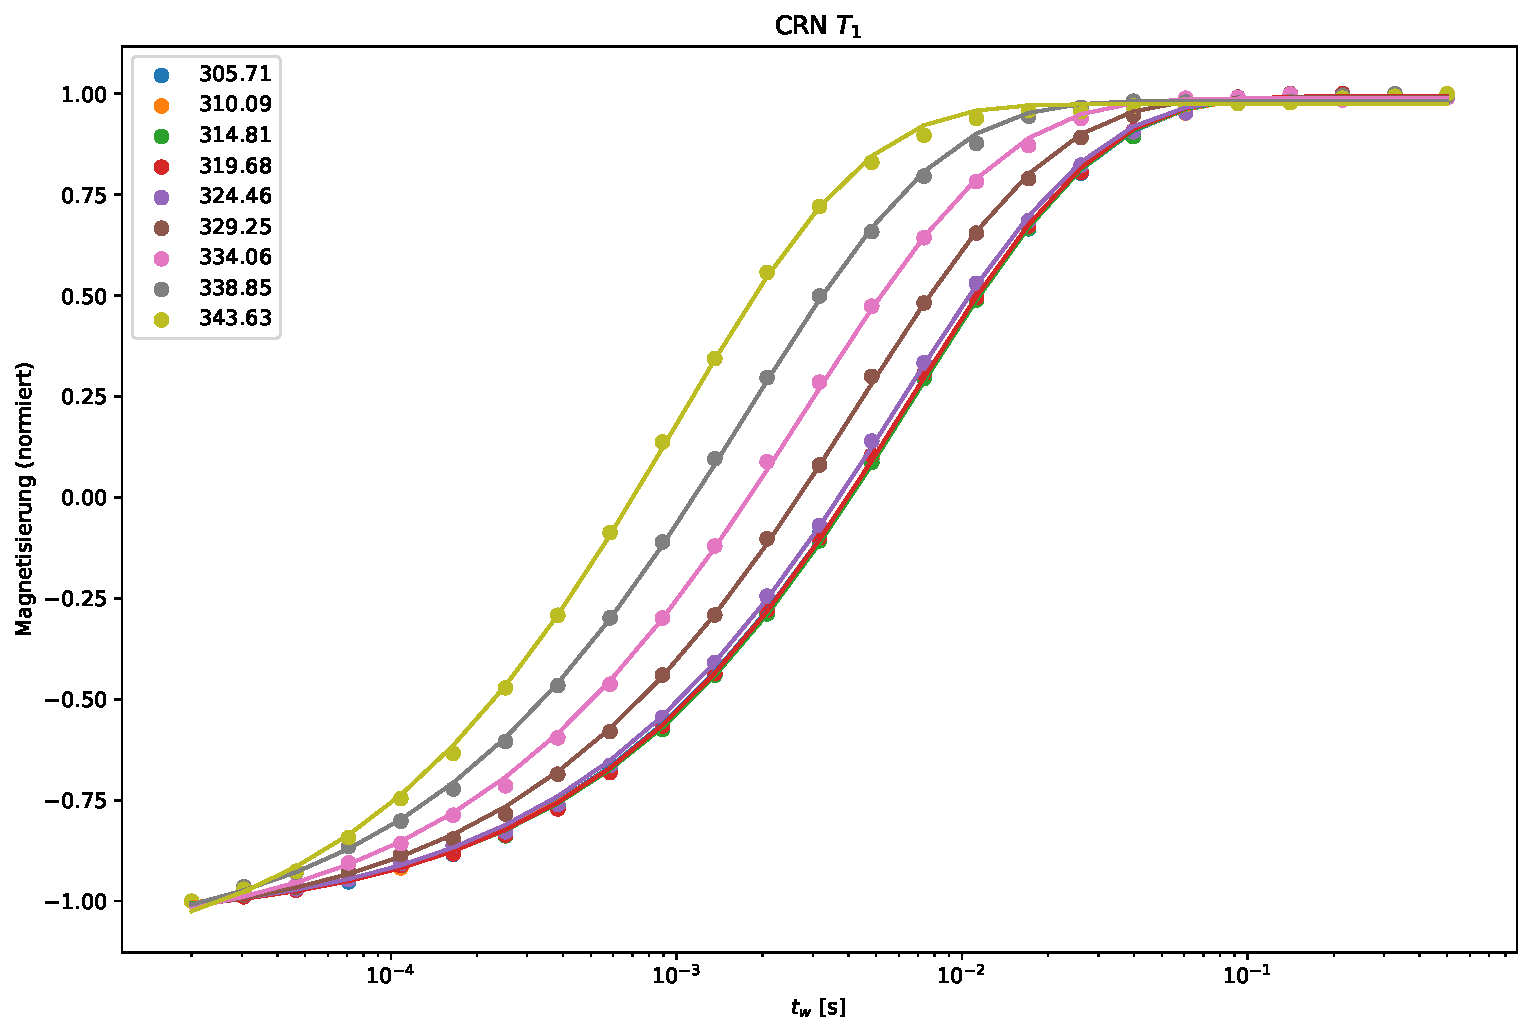
\includegraphics[width=\textwidth]{graphics/plots/T1/t1_roh.pdf}
	\end{center}
	\caption{$T_1$ Rohdaten} \label{fig:res:T_1_roh}
\end{figure}
Während sich die Kurven zwischen $\SI{305}{\kelvin}$ und $\SI{325}{\kelvin}$ sehr ähneln, verschieben sich die Kurven und damit auch die $T_1$-Werte bei höheren Temperaturen zu kürzeren Zeiten.

Dies lässt sich auch in der Gesamtübersicht aller aufgenommenen $T_1$-Daten in Abbildung \ref{fig:res:T_1} erkennen. Während die $T_1$-Zeiten bei Temperaturen von $\SI{250}{\kelvin}$ bis $\SI{325}{\kelvin}$ nahezu unverändert im unteren Millisekunden-Bereich liegen, verkürzen sie sich bei steigenden Temperaturen bis in den zweistelligen Mikrosekunden-Bereich. Es ist ein $T_1$-Minimum bei etwa $\SI{390}{\kelvin}$ auszumachen, ehe die $T_1$-Zeiten stagnieren oder sogar länger werden.

Während die Unsicherheiten weitestgehend vernachlässigbar sind, sind starke Schwankungen über $\SI{390}{\kelvin}$ zu erkennen. Die dort aufgenommenen Daten kann nicht mehr Bedeutung als einer groben Idee der Tatsachen zugemessen werden.

Abgesehen von dem erwähnten Temperaturbereich ist eine gute Übereinstimmung zu den $T_1$-Daten von Zürn \cite{zuern_paper} und zwischen Messungen mit überlappenden Temperaturbereichen zu erkennen, was darauf schließen lässt, dass diese Daten gut reproduzierbar sind.

\begin{figure}
	\begin{center}
		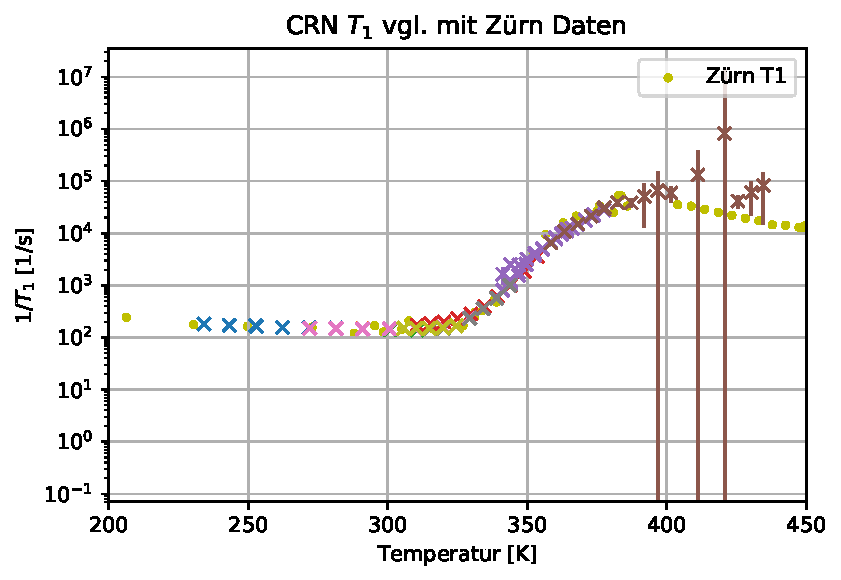
\includegraphics[width=\textwidth]{graphics/plots/T1/t1.pdf}
	\end{center}
	\caption{$T_1$ aus Fits nach Gleichung \eqref{eqn:theo:T_2_fit}. Unterschiedliche Farben indizieren hierbei gesonderte Messreihen; gelbe Punkte bieten einen Vergleich mit Daten von Zürn.} \label{fig:res:T_1}
\end{figure}

\begin{figure}
	\begin{center}
		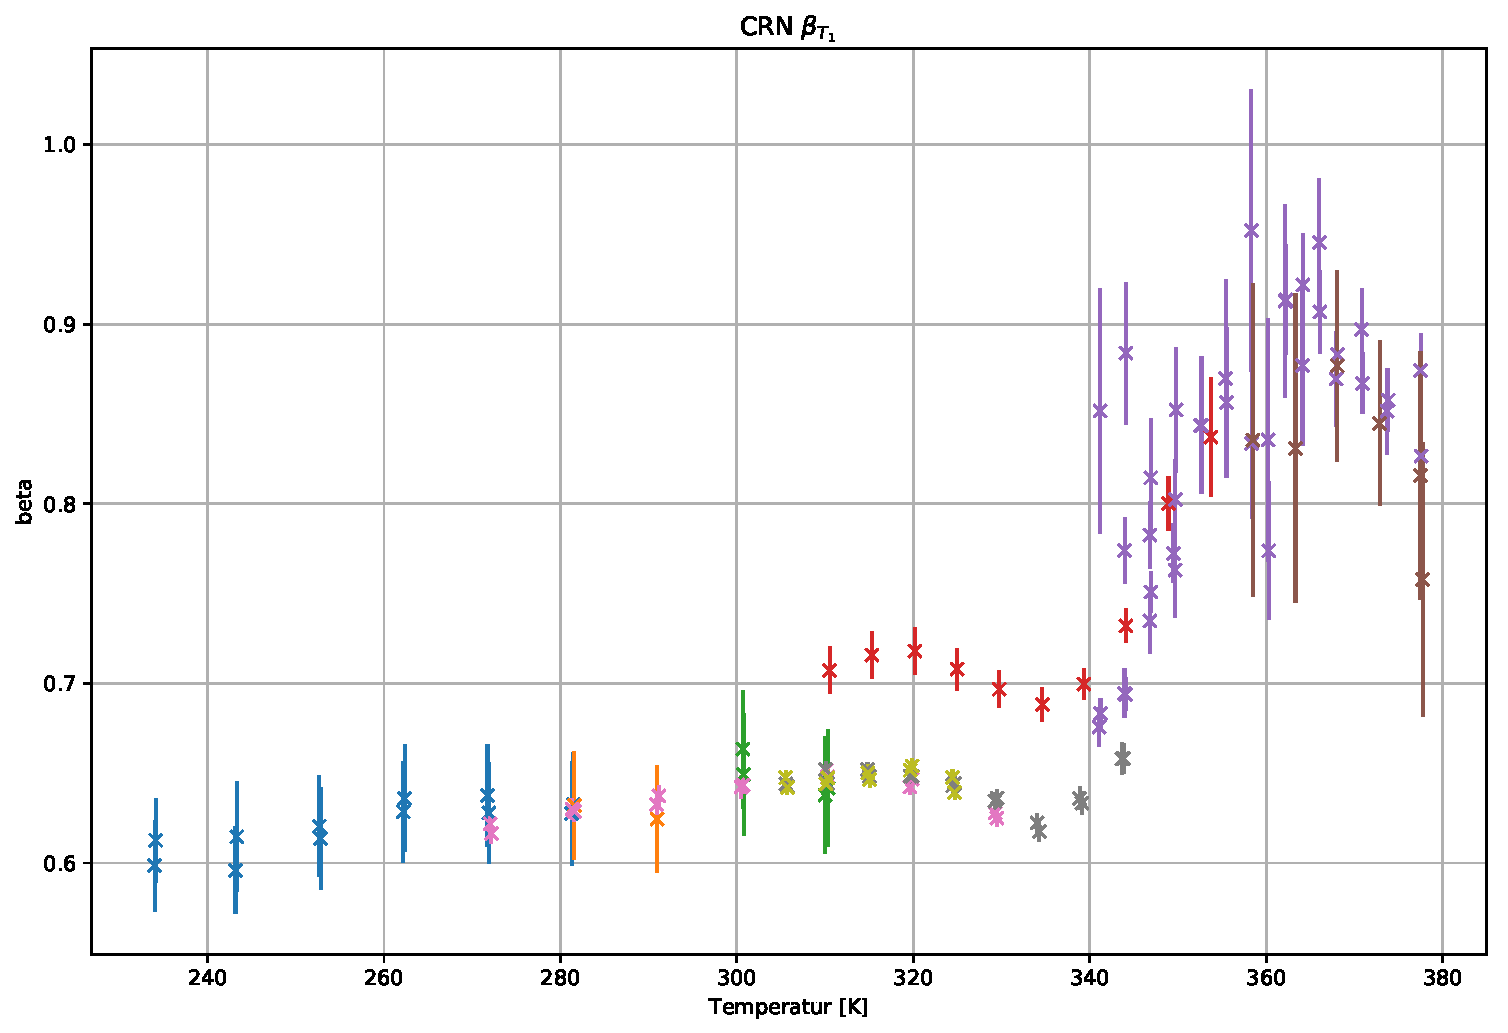
\includegraphics[width=\textwidth]{graphics/plots/T1/t1_beta.pdf}
	\end{center}
	\caption{$\beta_{T_1}$} \label{fig:res:beta_T_1}
\end{figure}
$\beta$ der Fits. Hohe Schwankung bei Temperaturen 340-380 K, da $T_1$ sehr kurz sich und dementsprechend die Signale klein. Temperaturen über 380K abgeschnitten, da Unsicherheit zu groß.


\section{$T_2$} \label{section:res:T_2}

\begin{figure}
	\begin{center}
		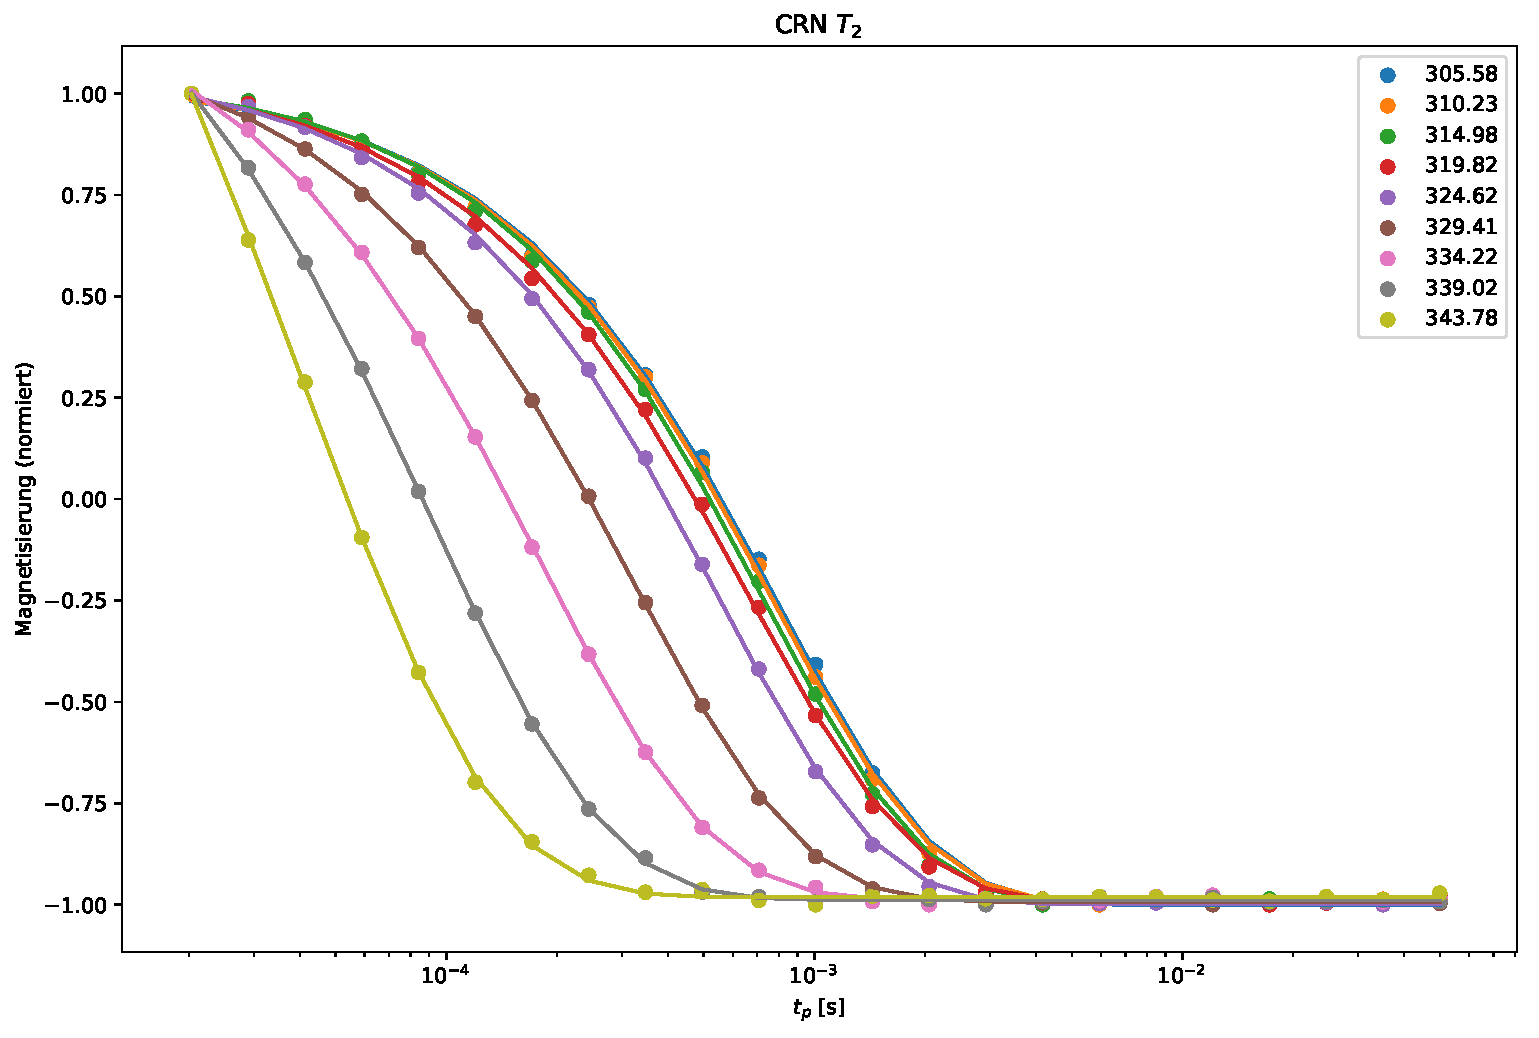
\includegraphics[width=\textwidth]{graphics/plots/T2/t2_roh.pdf}
	\end{center}
	\caption{$T_2$ Rohdaten} \label{fig:res:T_2_roh}
\end{figure}
Aufgenommen am OBI ($\SI{300}{MHz}$) mit Hahnecho, $\tau = \SI{15}{\micro s}$. Länge eines Pi-Pulses $\tau = \SI{7.6}{\micro s}$. Punkte sind Messwerte, Linien Fits mit Kohlrausch-Funktion.

\begin{figure}
	\begin{center}
		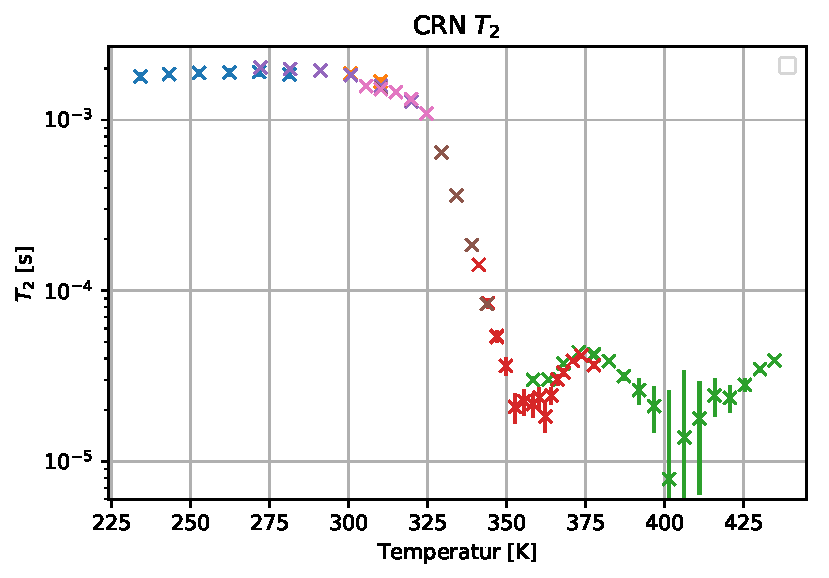
\includegraphics[width=\textwidth]{graphics/plots/T2/t2.pdf}
	\end{center}
	\caption{$T_2$ gegen Temperatur} \label{fig:res:T_2}
\end{figure}
Ergebnisse der Fits, hier die $\tau$s. Hohe Unsicherheit bei hohen Temperaturen wegen niedrigen $T_2$ und entsprechend kleinen Daten.

\begin{figure}
	\begin{center}
		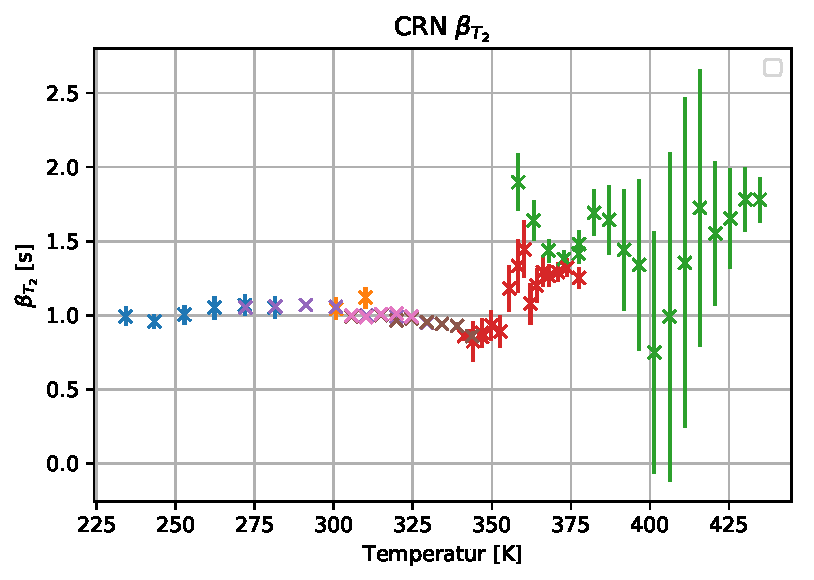
\includegraphics[width=\textwidth]{graphics/plots/T2/t2_beta.pdf}
	\end{center}
	\caption{$\beta_{T_2}$ gegen Temperatur} \label{fig:res:beta_T_2}
\end{figure}
Ergebnisse der Fits, hier die $\beta$. Hohe Unsicherheit bei hohen Temperaturen wegen niedrigen $T_2$ und entsprechend kleinen Daten.




\section{$F_2$} \label{section:res:F_2}

\begin{figure}
	\begin{center}
		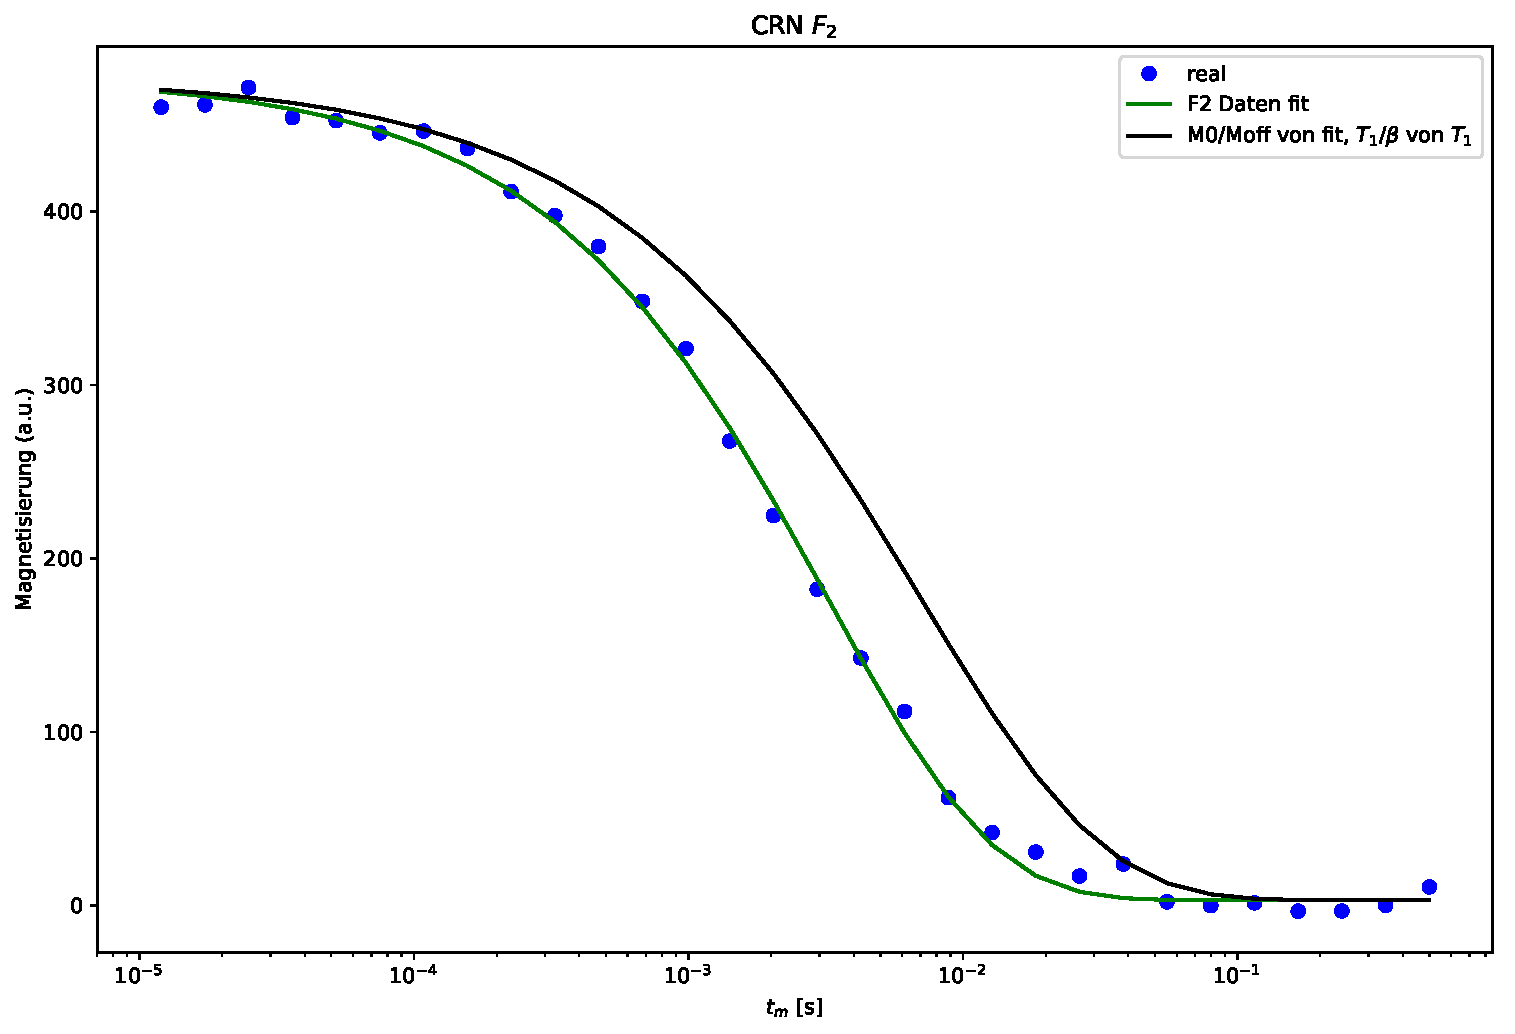
\includegraphics[width=\textwidth]{graphics/plots/F2/f2_fits.pdf}
	\end{center}
	\caption{$F_2$ Fits} \label{fig:res:F_2_fit}
\end{figure}
Aufgenommen am OBI ($\SI{300}{MHz}$) mit stimuliertem Echo Sin-Sin 3-Puls-Folge, Evolutionszeit $t_p = \SI{1}{\milli s}$. Punkte sind Messwerte, grüne Linie ist Kohlrausch-Fit an Messwerte, schwarze Linie der gleiche Fit, aber $\tau$ und $\beta$ ausgetauscht für $T_1$ und $\beta_{T_1}$ aus einer $T_1$-Messung. Dieses Vorgehen wurde gewählt, weil die Daten keinen Fit mit zwei $\tau$ gleichzeitig unterstützen, aber dennoch einen Unterschied zum reinen $T_1$ zeigen. Temperatur 310K


\begin{figure}
	\begin{center}
		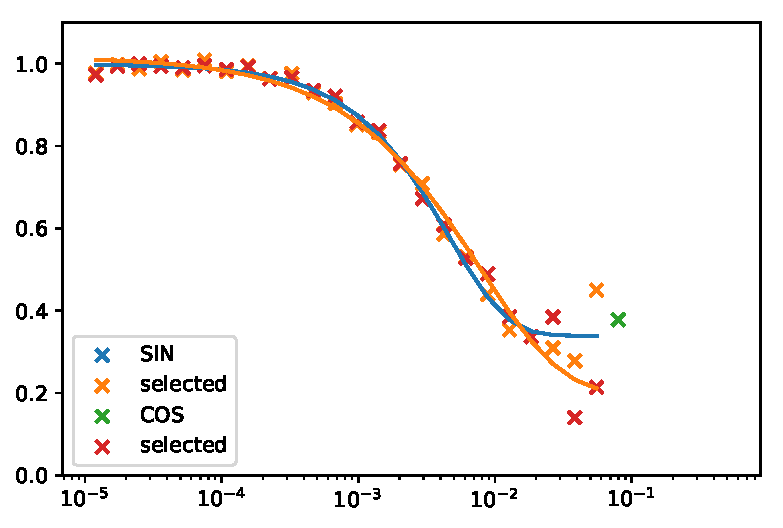
\includegraphics[width=\textwidth]{graphics/plots/F2/f2_fit.pdf}
	\end{center}
	\caption{$F_2$ geteilt durch Fit} \label{fig:res:F_2_T_1}
\end{figure}
Messdaten geteilt durch schwarze Linie. Bei Zeiten höher als mehrere Hundert ms schwanken die Daten stark (da ungefähr 0 durch 0 geteilt wird), daher werden sie abgeschnitten. An die Daten wird ein weiterer Kohlrausch-Fit gelegt. Sin-Sin und Cos-Cos zeigen sehr ähnliche Ergebnisse. Temperaturen 300K und 310K, Ergebnisse ähnlich.


\begin{figure}
	\begin{center}
		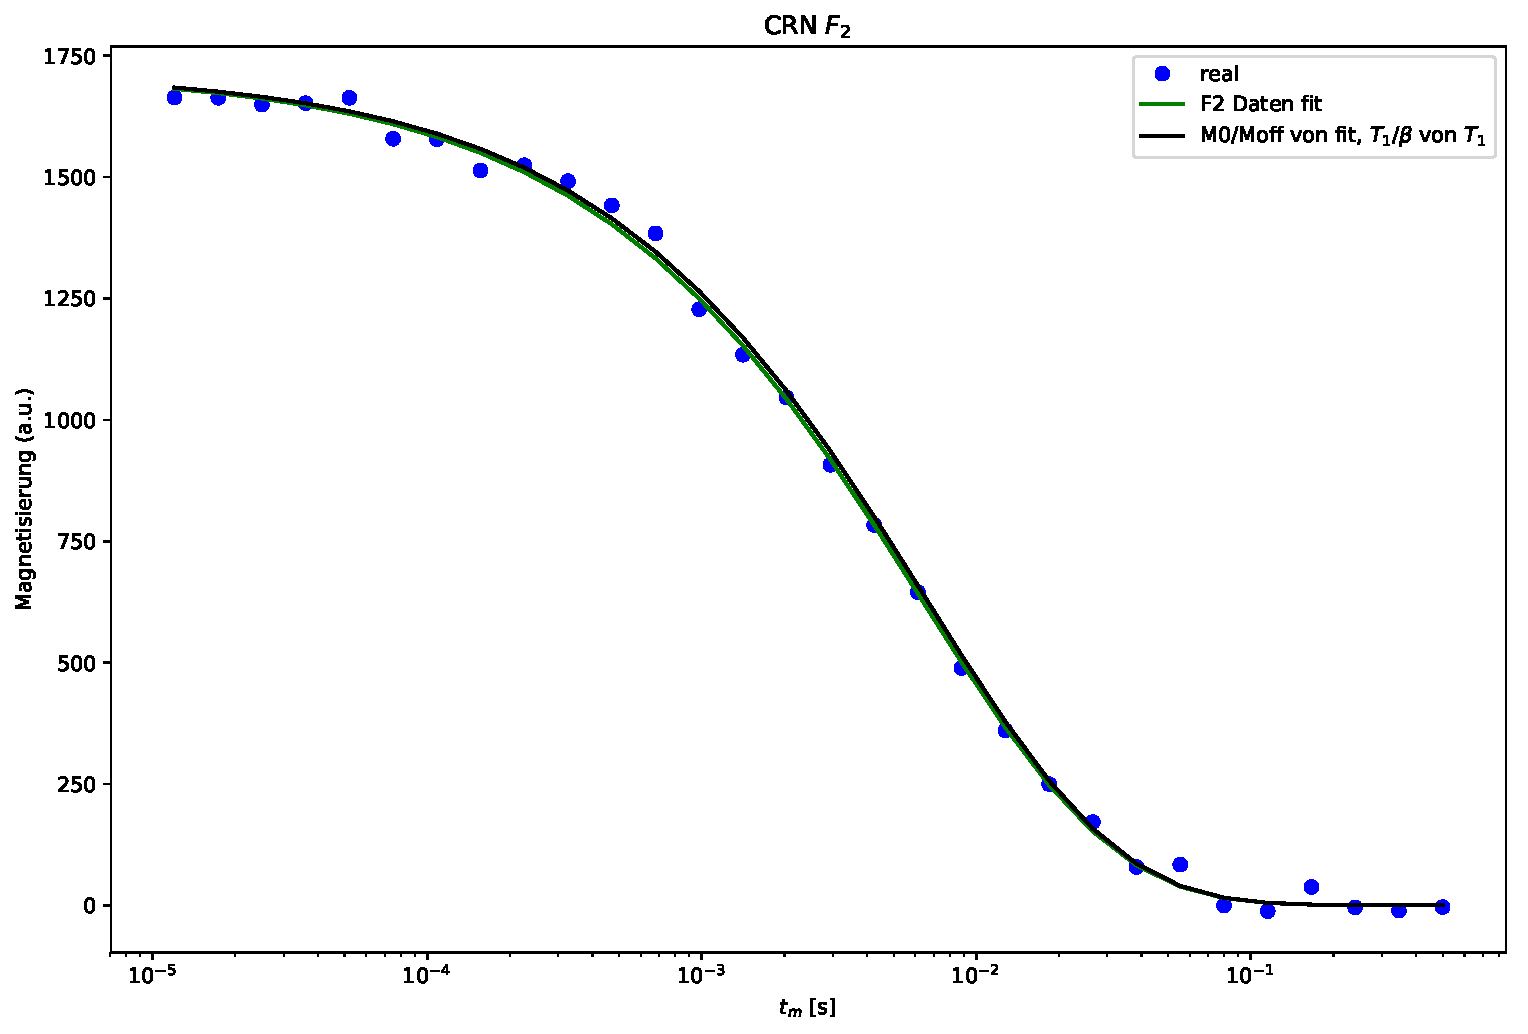
\includegraphics[width=\textwidth]{graphics/plots/F2/f2_tieftemp.pdf}
	\end{center}
	\caption{$F_2$ bei tiefen Temperaturen} \label{fig:res:F_2_tieftemp}
\end{figure}
Für tiefere Temperaturen (hier 280K) ist quasi kein Unterschied zwischen $F_2$ und $T_1$ zu erkennen.


\section{Spektren} \label{section:res:spektren}

\begin{figure}
	\begin{center}
		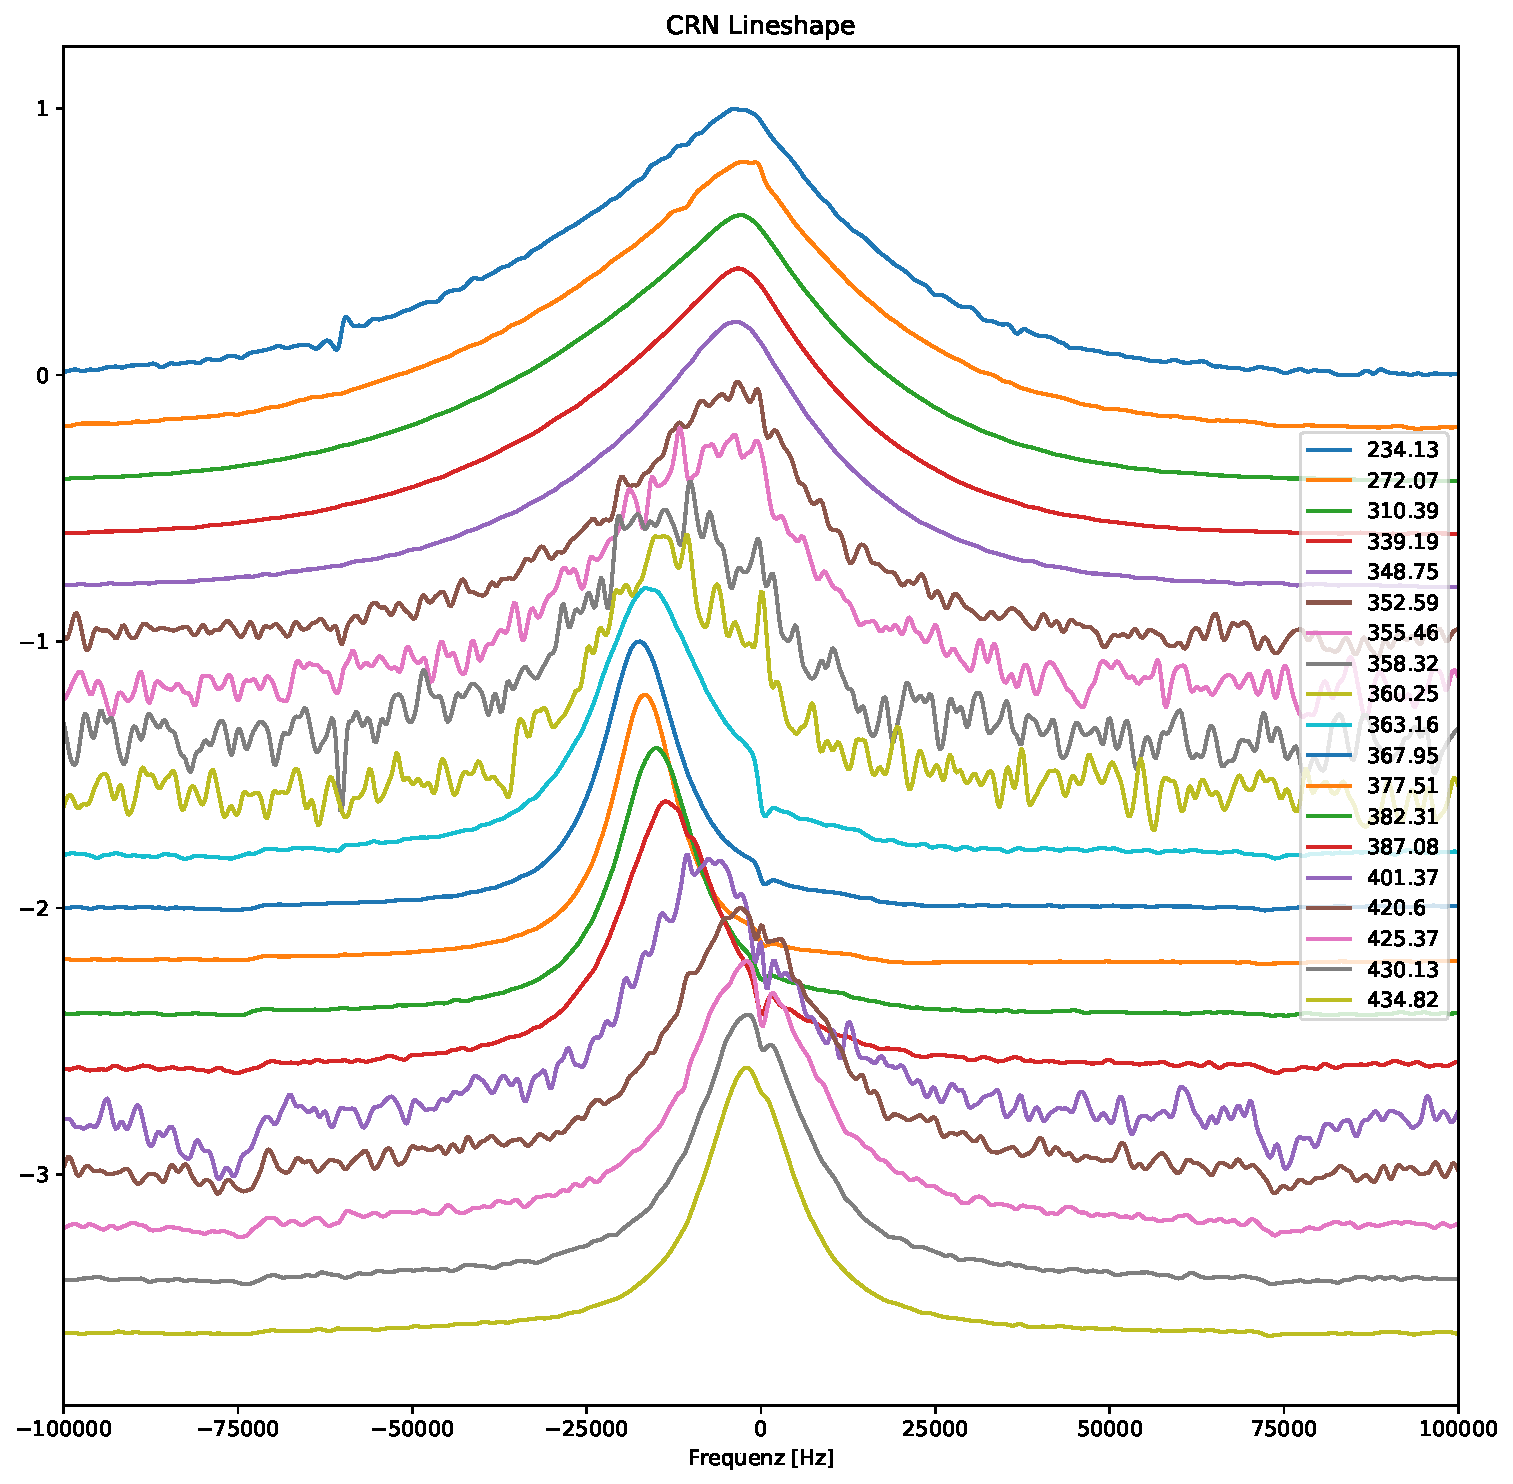
\includegraphics[width=\textwidth]{graphics/plots/SPEK/spek_lineshape.pdf}
	\end{center}
	\caption{Spektren Linienform} \label{fig:res:spek_linienform}
\end{figure}
Aufgenommen am OBI ($\SI{300}{MHz}$) mit Hahnecho, $\tau = \SI{15}{\micro s}$. Länge eines Pi-Pulses $\tau = \SI{7.6}{\micro s}$. Alle Spektren mit $\SI{500}{Hz}$ apodisiert.

Bei tiefen Temperaturen eine Czjzek-Form, die sich über weite Temperaturen (235K - 350K) fast unverändert so hält. Darüber ändert sich die Linienform, Lorentz ist ein guter Fit. Schwerpunkt verschiebt sich zu niedrigeren Frequenzen. Minimum ist bei 367K, darüber wird das Spektrum breiter, hat Maximum bei etwa 410K, ehe es wieder schmaler wird. Schwerpunkt verschiebt sich ab 375K wieder gegen 0, wo es ab 400K verweilt.


\begin{figure}
	\begin{center}
		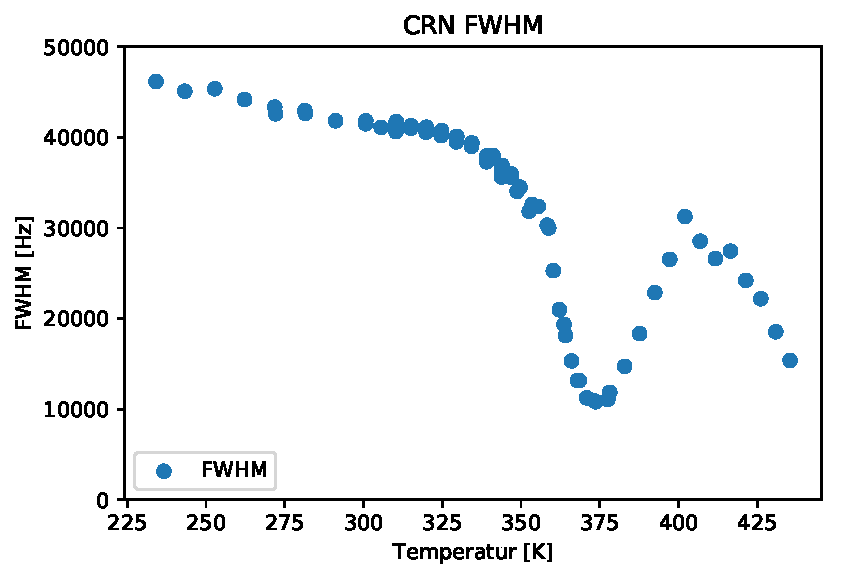
\includegraphics[width=\textwidth]{graphics/plots/SPEK/spek_fwhm.pdf}
	\end{center}
	\caption{Spektren FWHM} \label{fig:res:spek_fwhm}
\end{figure}
Um Beobachtungen zu quantisieren zwei Messgrößen: FWHM (Halbwertsbreite) und Schwerpunkt. Zwischen 350K und 360K sind die Spektren sehr verrauscht, ebenso bei 400K bis 420K; dort wurden Lorentz-Fits an die Spektren angelegt.


\begin{figure}
	\begin{center}
		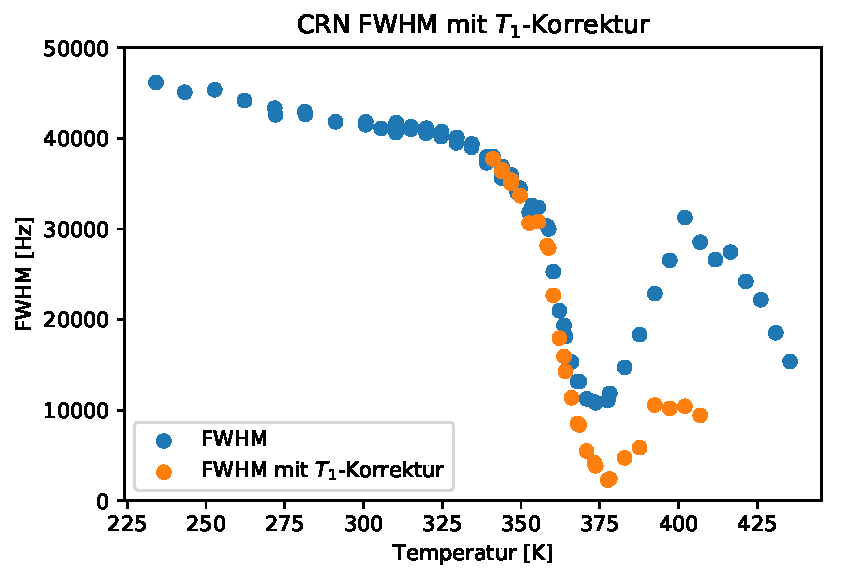
\includegraphics[width=\textwidth]{graphics/plots/SPEK/spek_t1korr.pdf}
	\end{center}
	\caption{Spektren FWHM mit $T_1$-Korrektur} \label{fig:res:spek_fwhm_t1}
\end{figure}
Aufgrund der Bewegungsverschmälerung würde man annehmen, dass die Halbwertsbreite sinkt, und nicht ein so hohes Maximum zeigt. Ein großer Einfluss ist die in dem Temperaturbereich (380K - 430K) sehr kurze $T_1$-Zeit. Durch den Einfluss von $T_1$ fällt das Signal sehr stark ab und verbreitert so das Spektrum.

Um den Einfluss von $T_1$ herauszurechnen: Die Spektren sind Fouriertransformierte der aufgenommenen Zeitsignale. Für die Spektren wird ein Lorentz 
\begin{align}
    L(f) = \frac{1}{\pi \gamma} \cdot \frac{\gamma^2}{\gamma^2 + (f - f_0)^2}
\end{align}
angenommen. Lorentz hat zwei Parameter, Maximum $f_0$ (und Schwerpunkt) und Halbwertsbreite $2\gamma$. Die Fouriertransformierte davon ist eine gedämpfte Schwingung:
\begin{align}
    h(t) = \exp{(-a |t|)} \cos{(2 \pi f_0 t)} \\
    H(t) = \int_{-\infty}^{\infty} h(t) \text{d} t \\
    H(f) = \frac{2}{a} \cdot \frac{(a/2\pi)^2}{((a/2\pi)^2) + (f - f_0)^2}
\end{align}
mit der Halbwertsbreite $\gamma = a/\pi$.

Das ursprüngliche Zeitsignal soll durch die $T_1$-Kurve geteilt werden, um den Einfluss herauszurechnen. Dafür werden ein Kohlrausch mit $\beta = 1$ angenommen, damit sich die Rechnung einfacher gestaltet:
\begin{align}
    f(t) = \exp{(-t/T_1)^\beta}
\end{align}
, die $T_1$-Werte stammen aus $T_1$-Messungen bei gleicher Temperatur. 

Fouriertransformiert ergibt sich die modifizierte Halbwertsbreite $2\gamma = 2(\gamma_0 - \frac{1}{\pi T_1})$.

Übrig bleibt ein kleinerer Peak (-> Theorie). Bei Temperaturen über 410K konnte keine Korrektur vorgenommen werden, weil die $T_1$-Werte da zu stark streuen.


\begin{figure}
	\begin{center}
		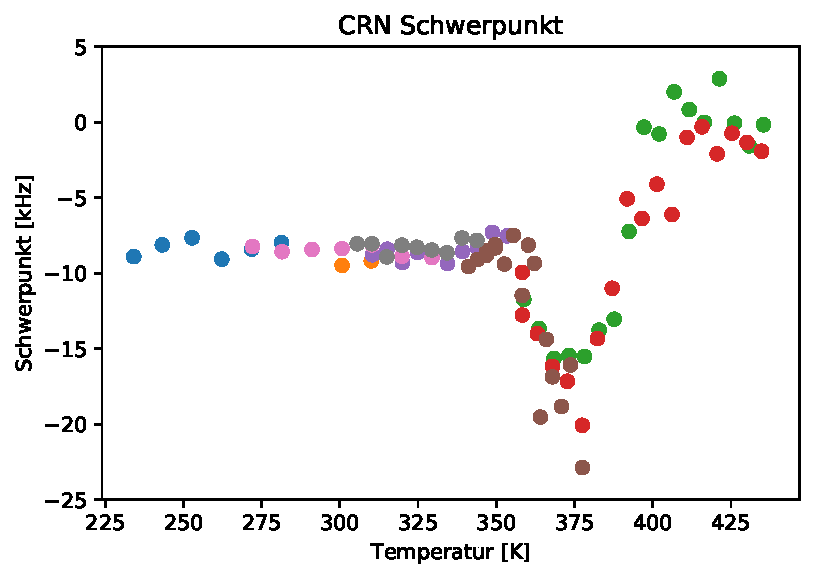
\includegraphics[width=\textwidth]{graphics/plots/SPEK/spek_mean.pdf} 
	\end{center}
	\caption{Spektren Schwerpunkt} \label{fig:res:spek_mean}
\end{figure}
Schwerpunkte; bei den stark verrauschten Spektren wurden die Werte wieder aus Lorentz-Fits bestimmt.


\section{Simulation} \label{section:res:sim}

\begin{figure}
	\begin{center}
		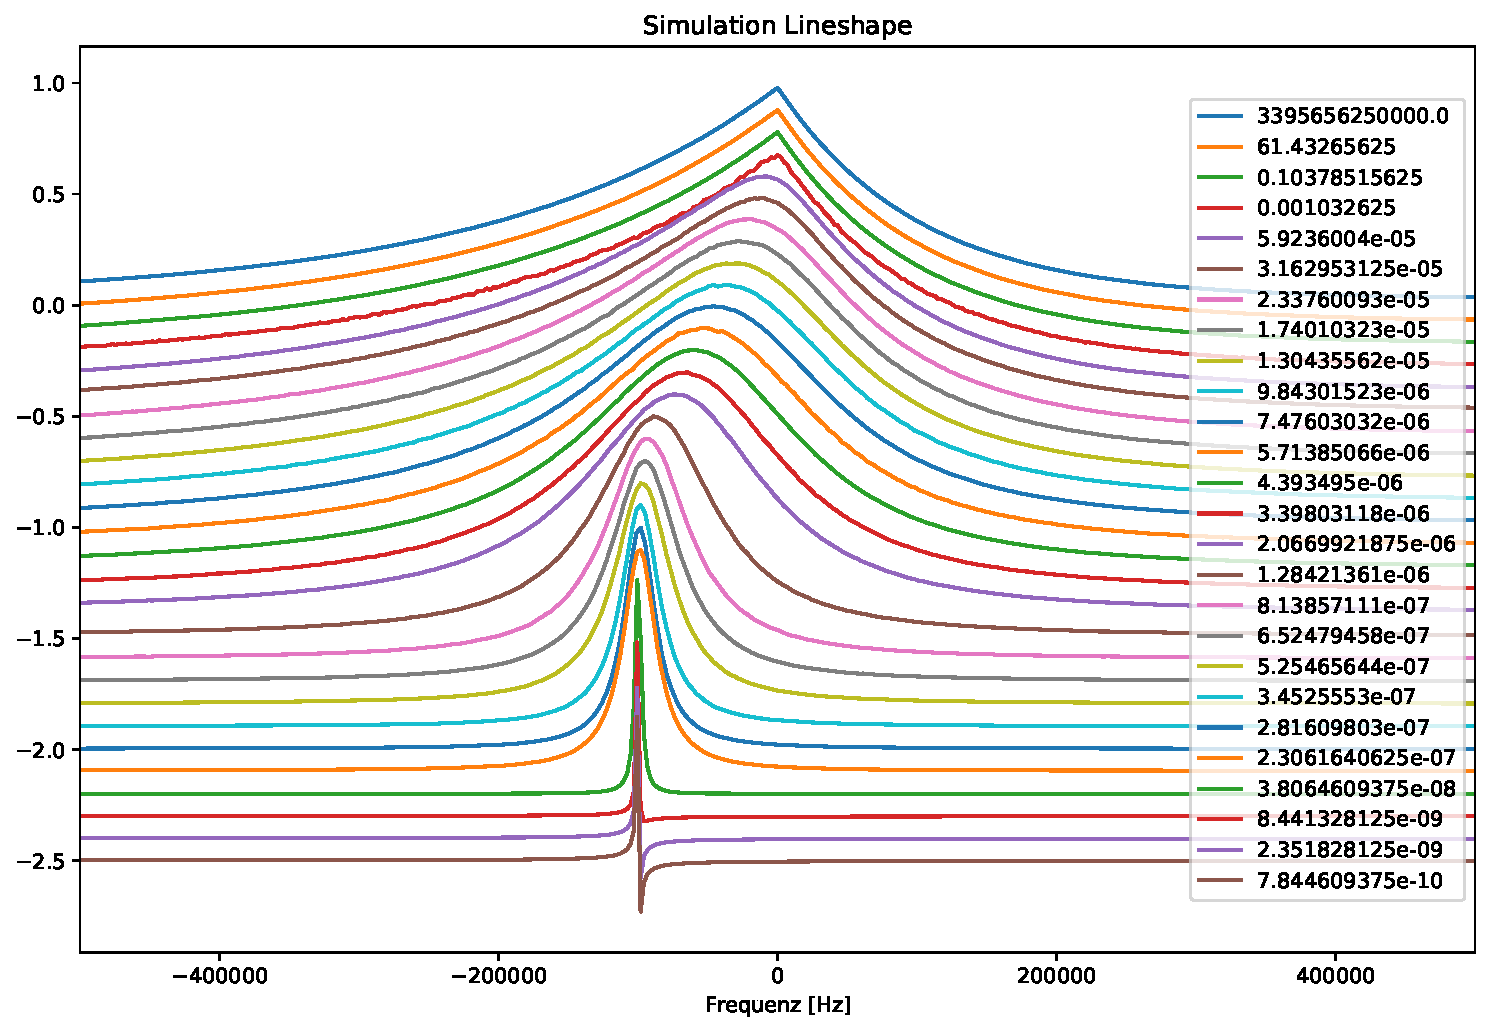
\includegraphics[width=\textwidth]{graphics/plots/SIM/sim_lineshape.pdf}
	\end{center}
	\caption{Simulation Linienform} \label{fig:res:sim_linienform}
\end{figure}
Das Verhalten der Linienform der Spektren sollte mit Random-Walk-Simulationen untersucht werden. Dazu wurde ein isotroper Zufallssprung verwendet. Ausgangsverteilung wurde zufällig aus Czjzek-Verteilung gezogen. Es wurde ein FID simuliert, Wechselwirkung war Quadrupol-WW 2. Ordnung. Dwelltime (Zeit zwischen zwei Samples): $\SI{0.5}{\micro s}$). Lebenszeiten der Zustände sind exponentiell verteilt, es wird ein Erwartungswert angegeben. Aus diesem wird mit Vogel-Fulcher-$\tau_{c}$ mit Werten aus dem 4er-Papier die Temperatur bestimmt. Andere $\tau_c$s, zum Beispiel aus DOI: 10.1103/PhysRevE.81.051504 zeigen keinen großen Unterschied.

Die Linienform sieht der des Experiments recht ähnlich, nur zu hohen Temperaturen werden die Spektren immer schmaler, anstatt wieder breiter zu werden. 

\begin{figure}
	\begin{center}
		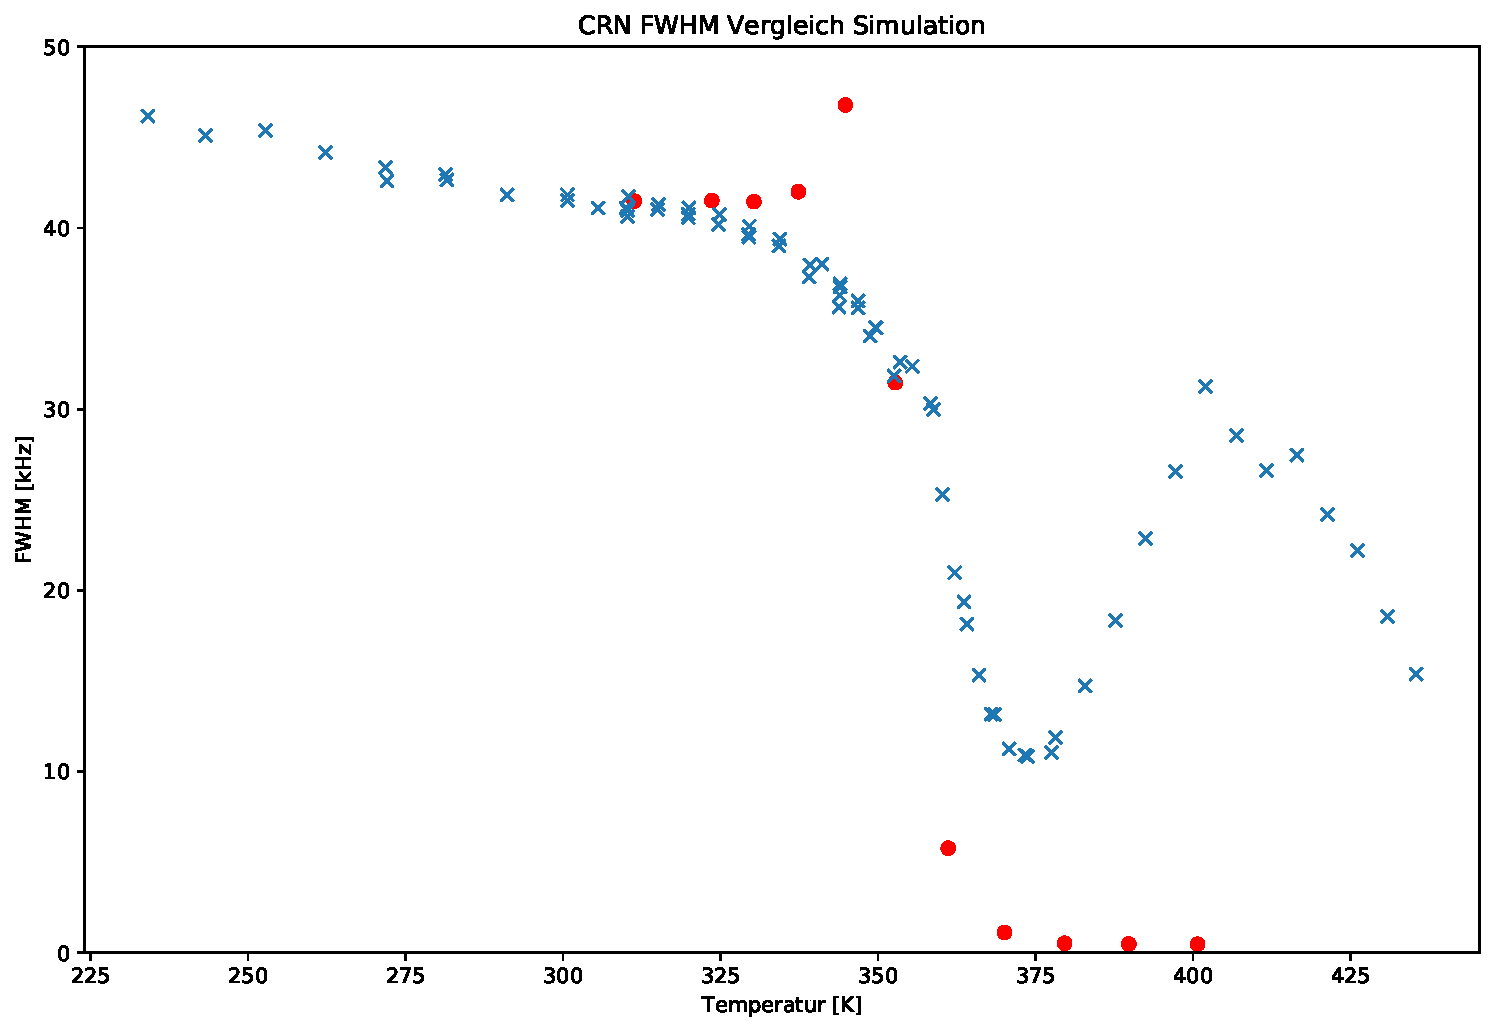
\includegraphics[width=\textwidth]{graphics/plots/SIM/sim_fwhm.pdf}
	\end{center}
	\caption{Simulation FWHM} \label{fig:res:sim_fwhm}
\end{figure}
Zusätzlich zeigt die Halbwertsbreite einen Peak bei ca. 350K. Dies kann daran liegen, dass hier der Übergang von der Czjzek-Form mit einer Spitze zur abgerundeten Lorentz-Form ist. Das Abrunden verschiebt die halbe Höhe zu niedrigeren Werten, daher der Peak. Die experimentellen Spektren zeigen aufgrund von Störungen auch bei niedrigeren keine perfekte Spitze und daher auch keinen Peak in der Halbwertsbreite beim Übergang.


% \begin{figure} % ***
% 	\begin{center}
% 		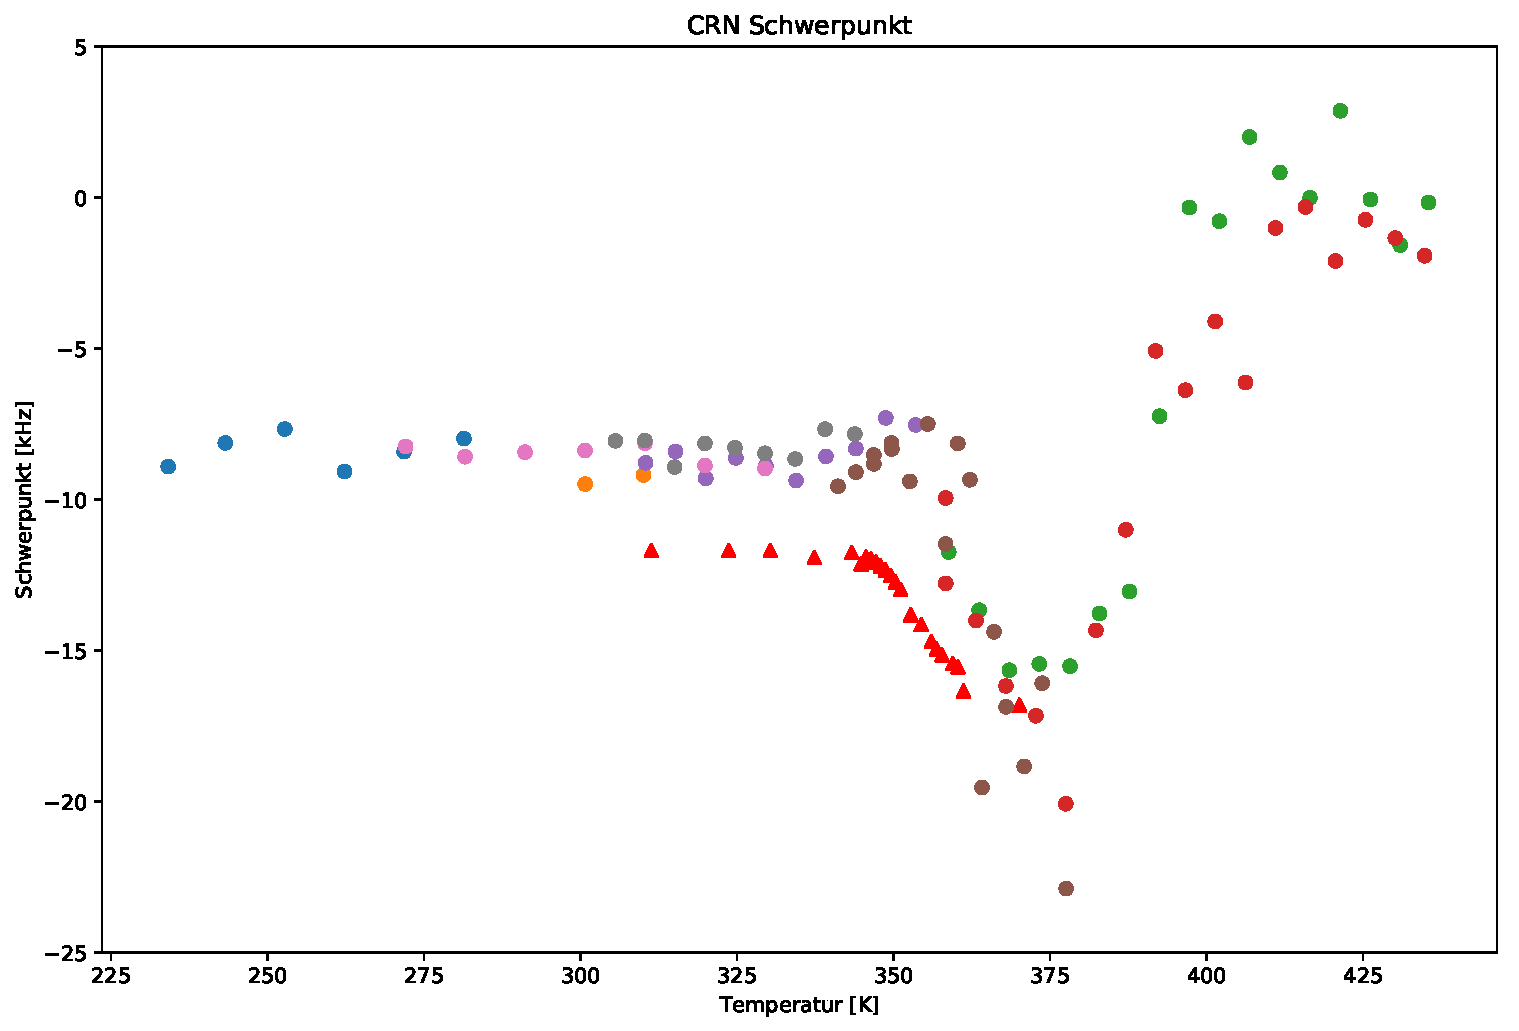
\includegraphics[width=\textwidth]{graphics/plots/SIM/sim_mean.pdf} 
% 	\end{center}
% 	\caption{Simulation Schwerpunkt} \label{fig:res:sim_mean}
% \end{figure}



\section{Theorie} \label{section:res:theorie}

Die experimentellen Ergebnisse sollen mit den theoretischen Überlegungen vergleichen werden.

\begin{figure}
	\begin{center}
		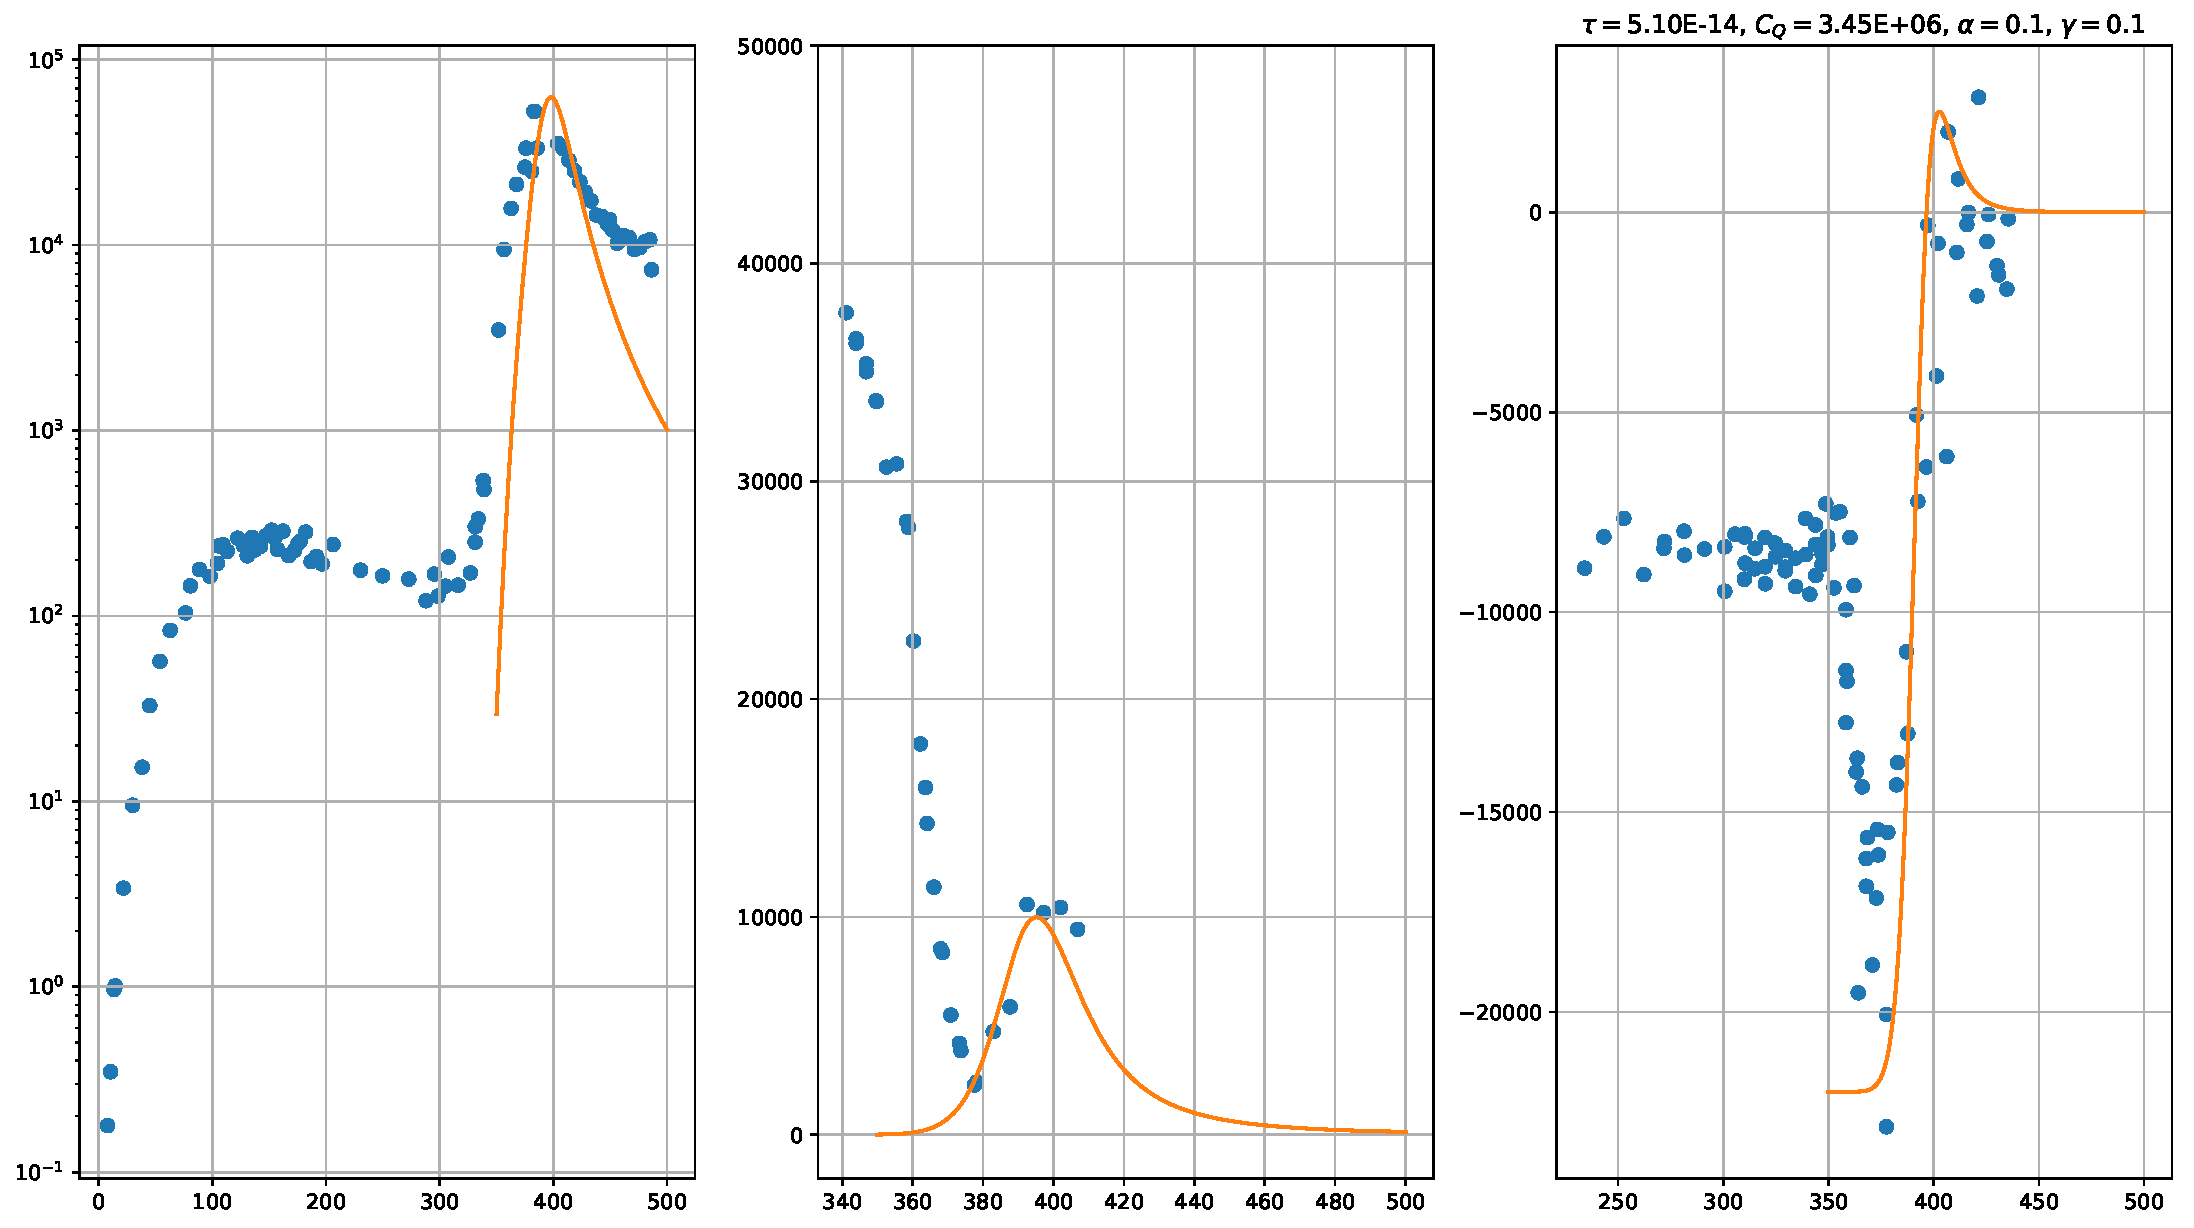
\includegraphics[width=\textwidth]{graphics/plots/THEO/J_01.pdf}
	\end{center}
	\caption{Spektraldichte $J$} \label{fig:res:theorie_j}
\end{figure}
Es werden verschiedene Spektraldichten verwendet, hier zuerst BPP. $\tau_c$ stammt aus dem 4er-Papier.

Für $C_Q = \SI{3.45}{MHz}$ gibt es eine gute Übereinstimmung für die $T_1$-bereinigte Halbwertsbreite und den Schwerpunkt, bei $T_1$ stimmt die grobe Form, bei den Flanken gibt es starke Abweichungen.

Mit $J_{CC}$ lässt sich mit $C_Q = \SI{3.65}{MHz}$ und $\alpha = 0.64$ $T_1$ gut abbilden, aber es gibt große Abweichungen bei der Halbwertsbreite. 

$J_{DC}$ ist mit $C_Q = \SI{3.2}{MHz}$ und $\gamma = 1.12$ ein Kompromiss in die andere Richtung, Schwerpunkt und Halbwertsbreite scheinen zu passen, aber bei $T_1$ gibt es wieder Abweichungen. 

Bei den Schwerpunkten von $J_{CC}$ und $J_{DC}$ ist noch zu klären, ob die verwendete Funktion für den Imaginärteil der Spektraldichte korrekt ist.

Alle drei Spektraldichten zeigen zwar gute, aber keine perfekten Übereinstimmungen mit den experimentellen Daten.



\begin{figure}
	\begin{center}
		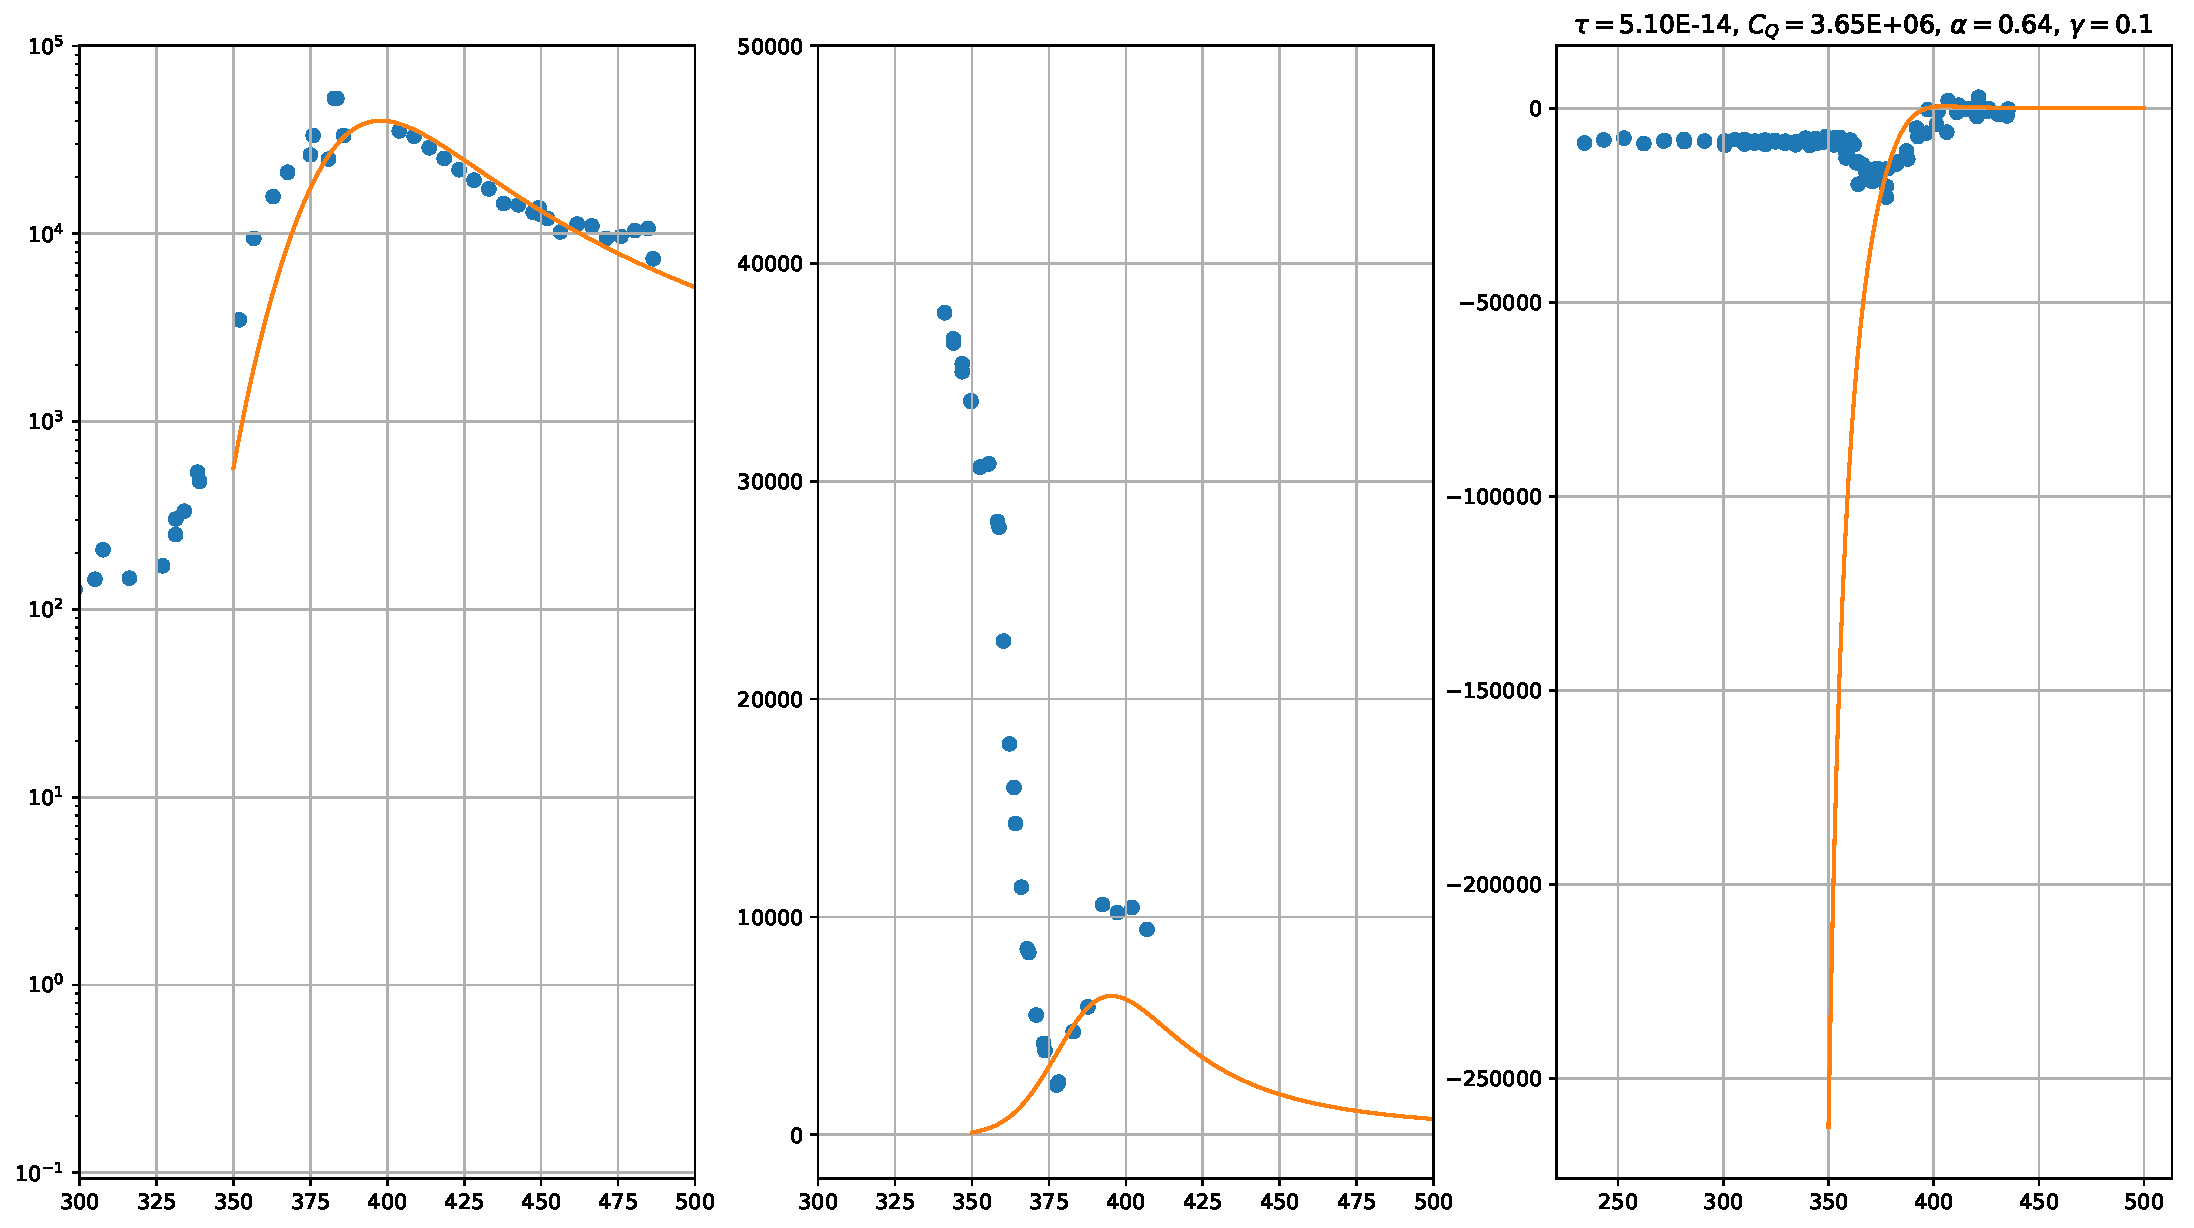
\includegraphics[width=\textwidth]{graphics/plots/THEO/J_cc_02.pdf}
	\end{center}
	\caption{Spektraldichte $J_{CC}$} \label{fig:res:theorie_j_cc}
\end{figure}

\begin{figure}
	\begin{center}
		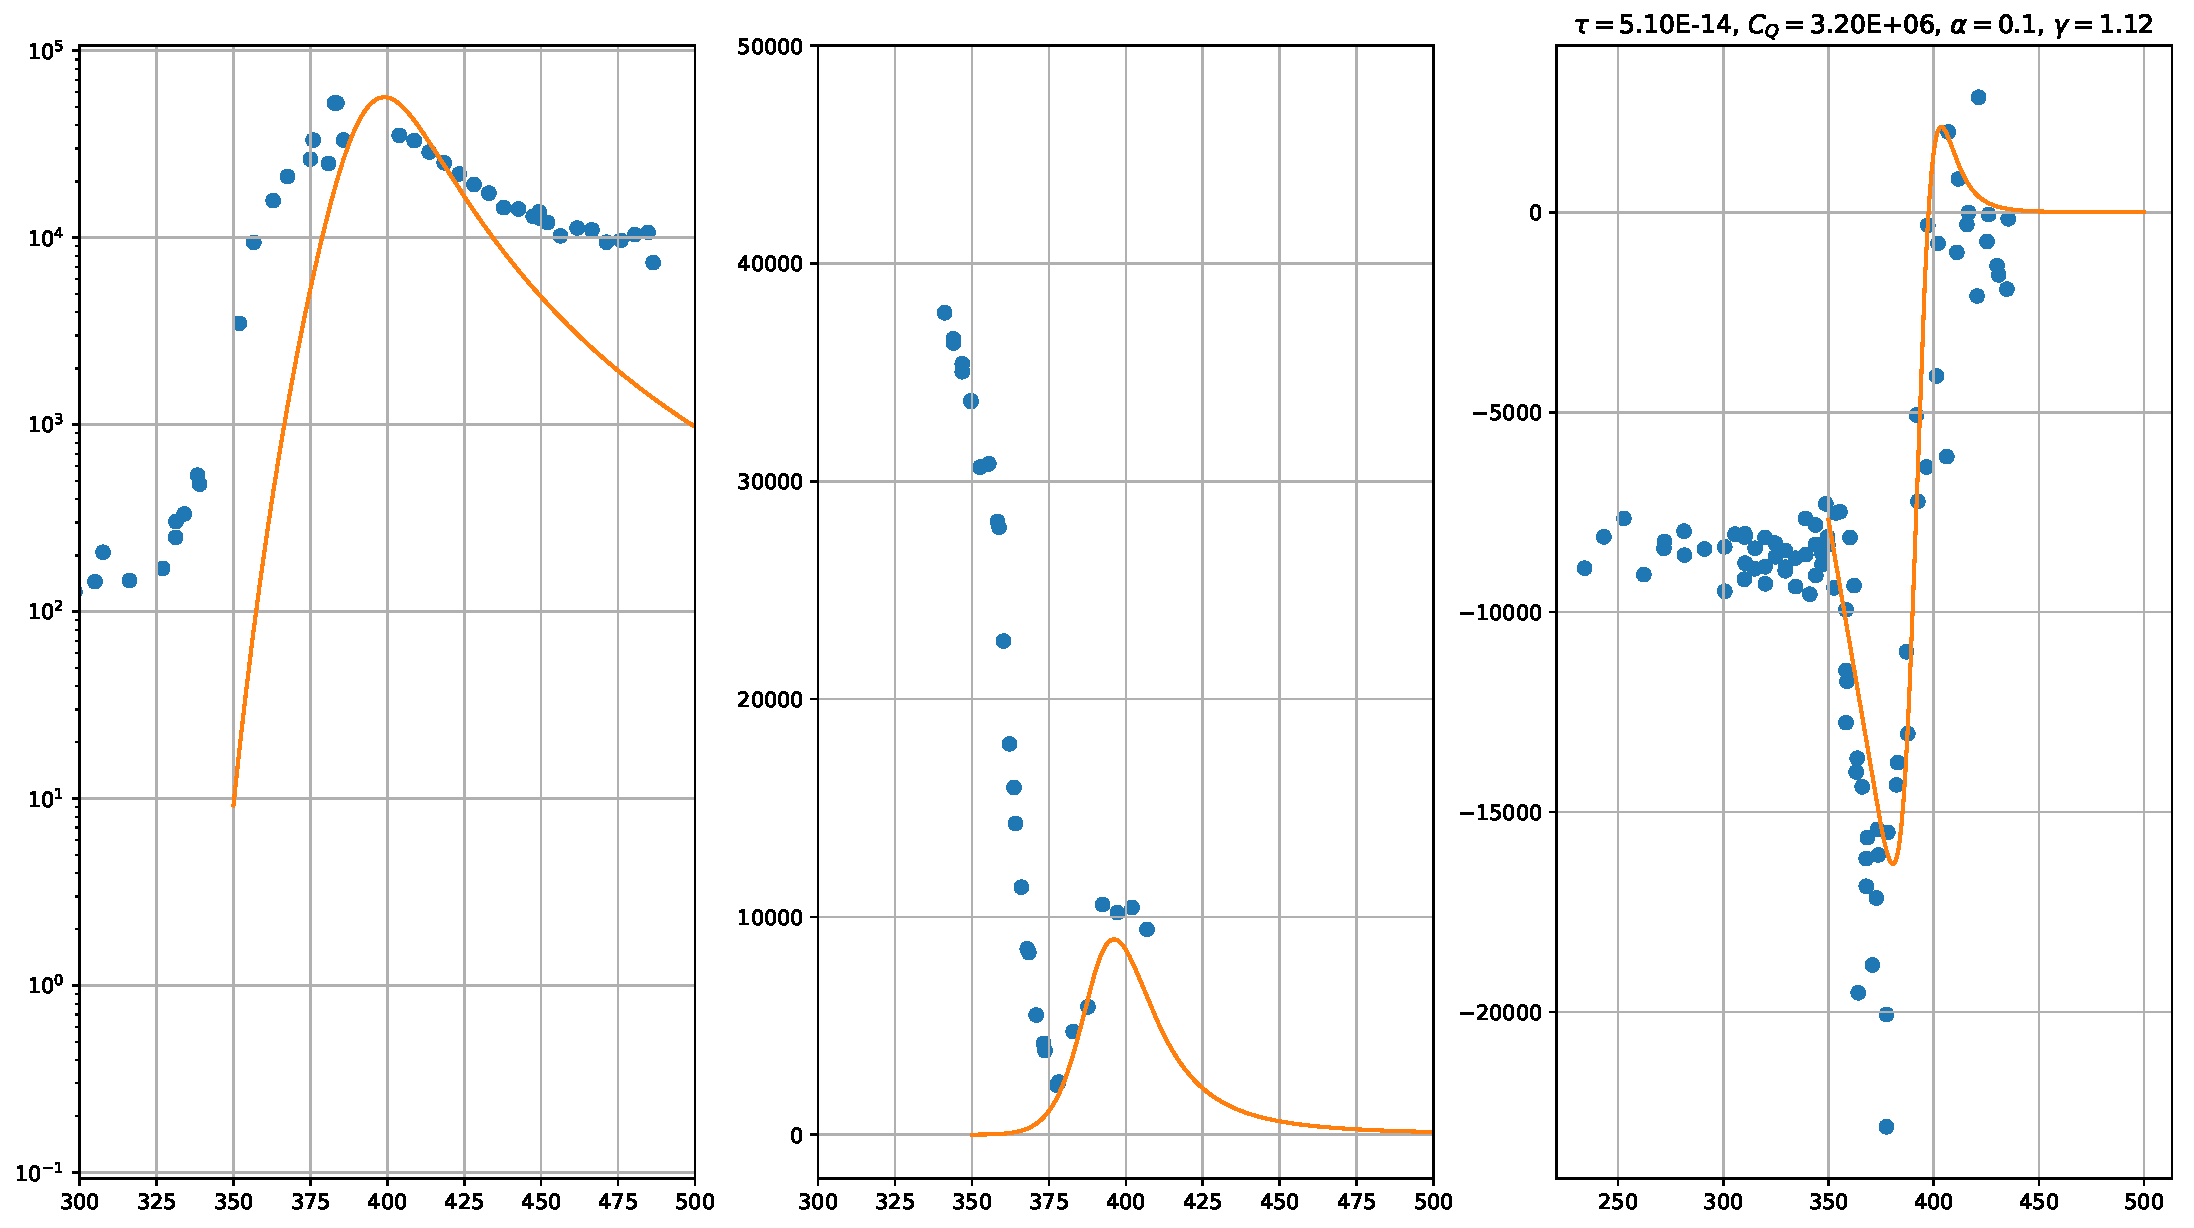
\includegraphics[width=\textwidth]{graphics/plots/THEO/J_dc_01.pdf}
	\end{center}
	\caption{Spektraldichte $J_{DC}$} \label{fig:res:theorie_j_dc}
\end{figure}




\section{Spektren Dynamik} \label{section:res:spekdyn}

Werden pulslängenabhängige Spektren aufgenommen, zeigt sich für unterschiedliche Temperaturen (hier beispielshaft 305K und 325K) ein unterschiedliches Verhalten der Linienform. Diese Tatsache soll verwendet werden, um an Information über die Dynamik zu kommen, die der Lienienformänderung zugrunde liegt.

\begin{figure}
	\begin{center}
		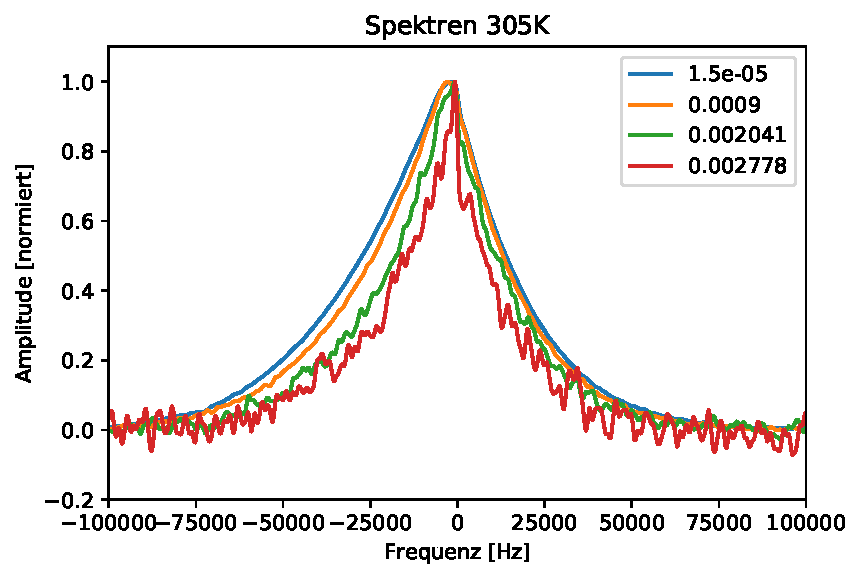
\includegraphics[width=\textwidth]{graphics/plots/SPEKDYN/spekdyn_305K.pdf}
	\end{center}
	\caption{Spektren Linienform($\tau$) 305K} \label{fig:res:spekdyn_305K}
\end{figure}

\begin{figure}
	\begin{center}
		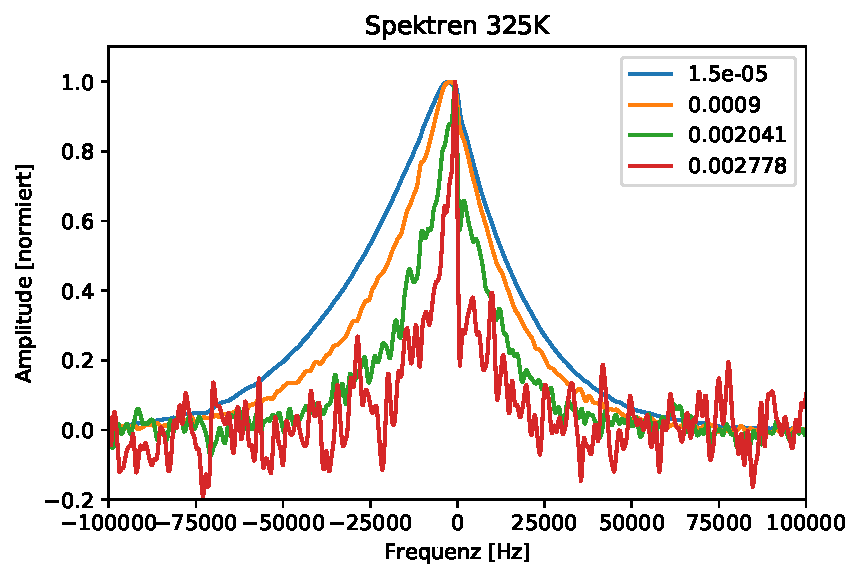
\includegraphics[width=\textwidth]{graphics/plots/SPEKDYN/spekdyn_325K.pdf}
	\end{center}
	\caption{Spektren Linienform($\tau$) 325K} \label{fig:res:spekdyn_325K}
\end{figure}

Dafür wird wird die Halbwertsbreite gegen die Pulslänge aufgetragen. Da die Spektren bei hohen Pulslängen teils sehr verrauscht sind, wurden hier für tiefe Temperaturen die Pulslängen auf $t_p = \SI{2}{\milli s}$ beschränkt.
\begin{figure}
	\begin{center}
		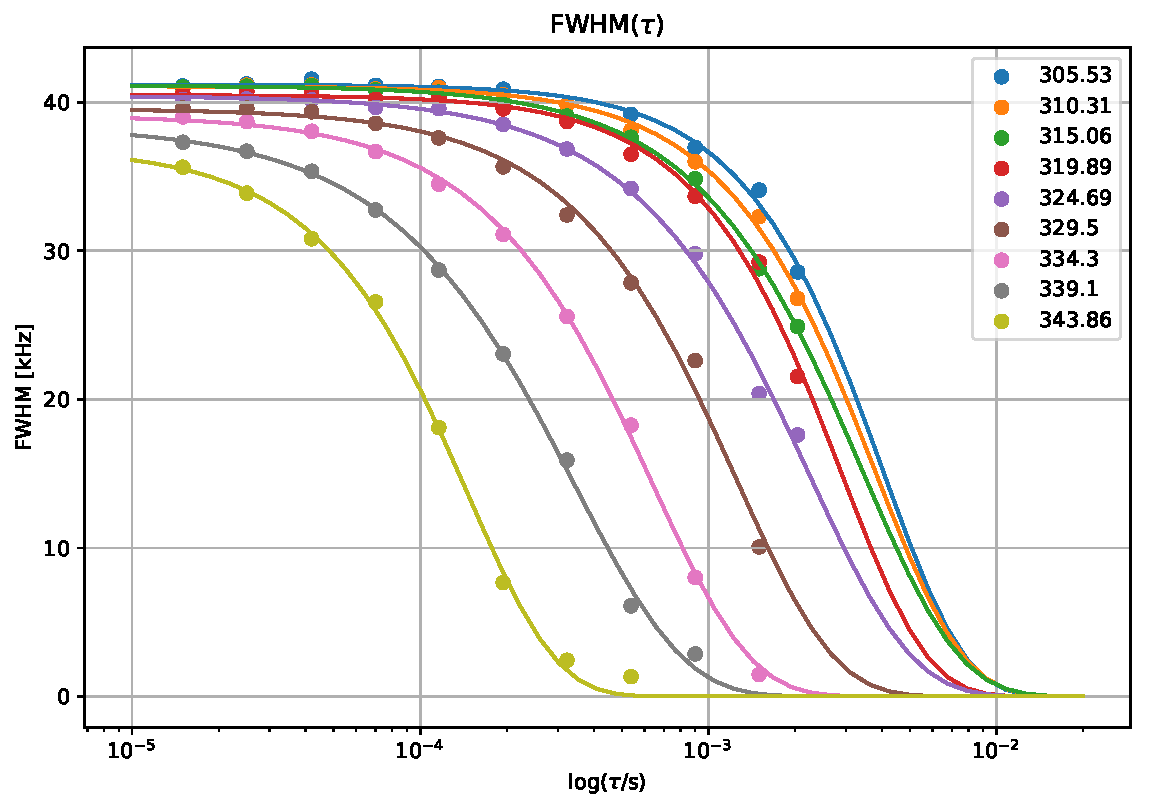
\includegraphics[width=\textwidth]{graphics/plots/SPEKDYN/spekdyn_fits.pdf}
	\end{center}
	\caption{FWHM Fits} \label{fig:res:spekdyn_fits}
\end{figure}
An die mit Punkten dargestellten Daten wurde ein Kohlrausch-Fit angelegt, gezeigt als durchgezogene Linie.

Werden die resultierenden Zeitkonstanten zusammen mit $T_2$ aufgetragen, zeigt sich eine hohe Ähnlichkeit, was vermuten lässt, dass mit der Methode $T_2$ gemessen wurde.
\begin{figure}
	\begin{center}
		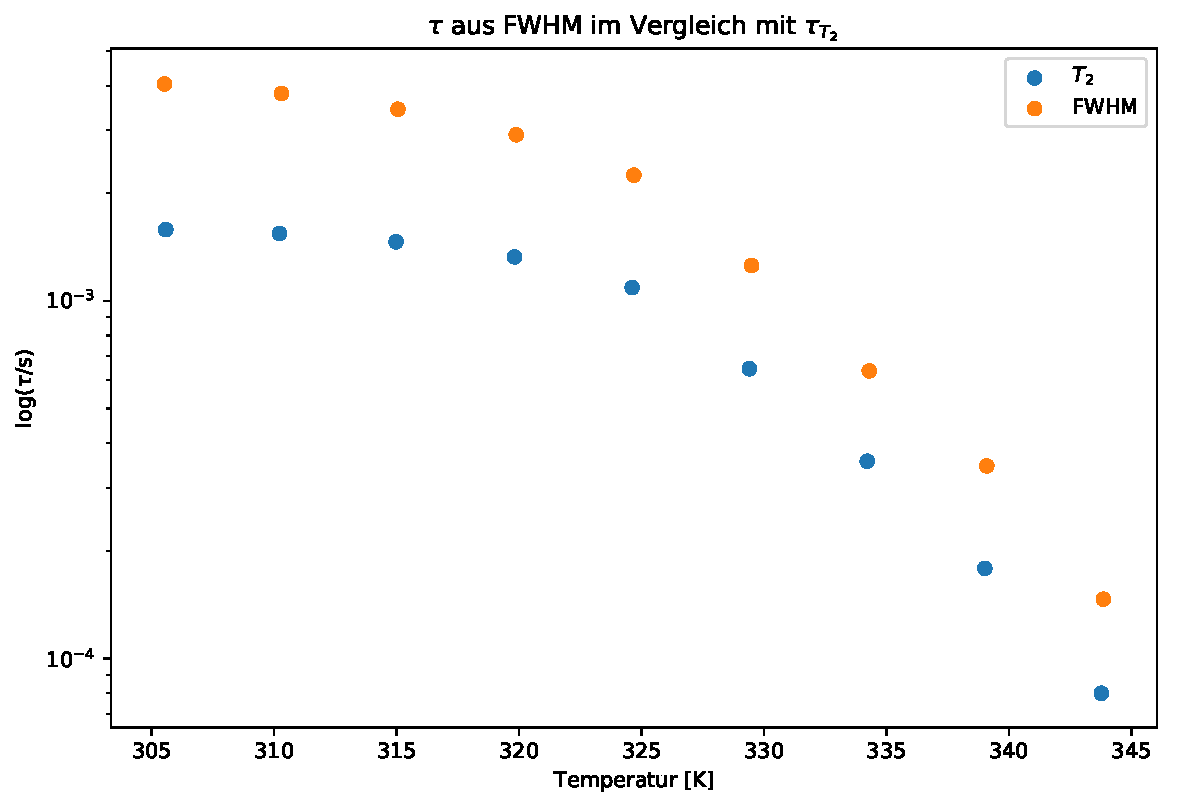
\includegraphics[width=\textwidth]{graphics/plots/SPEKDYN/spekdyn_t2.pdf}
	\end{center}
	\caption{$\tau$ aus FWHM im Vergleich mit $T_2$} \label{fig:res:spekdyn_t2}
\end{figure}



\section{Bruker} \label{section:res:bruker}

Neben dem $\SI{300}{MHz}$-Spektrometer wurden auch einige Messungen an einem $\SI{400}{MHz}$ Spektrometer von Bruker durchgeführt.
\begin{figure}
	\begin{center}
		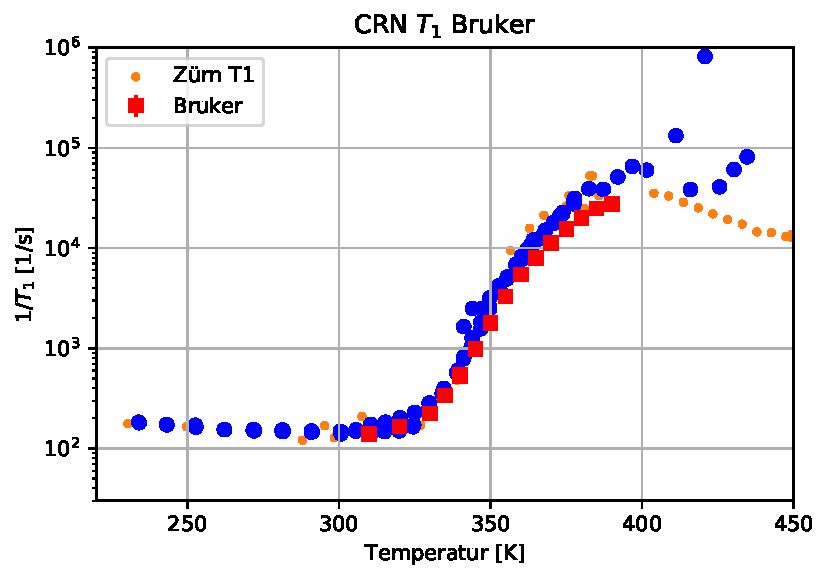
\includegraphics[width=\textwidth]{graphics/plots/BRUKER/bruker_t1.pdf}
	\end{center}
	\caption{Bruker $T_1$} \label{fig:res:bruker_t1}
\end{figure}
Die $T_1$-Werte und die dazugehörigen $\beta$ zeigen gute Übereinstimmung zu den anderen Daten auf.
\begin{figure}
	\begin{center}
		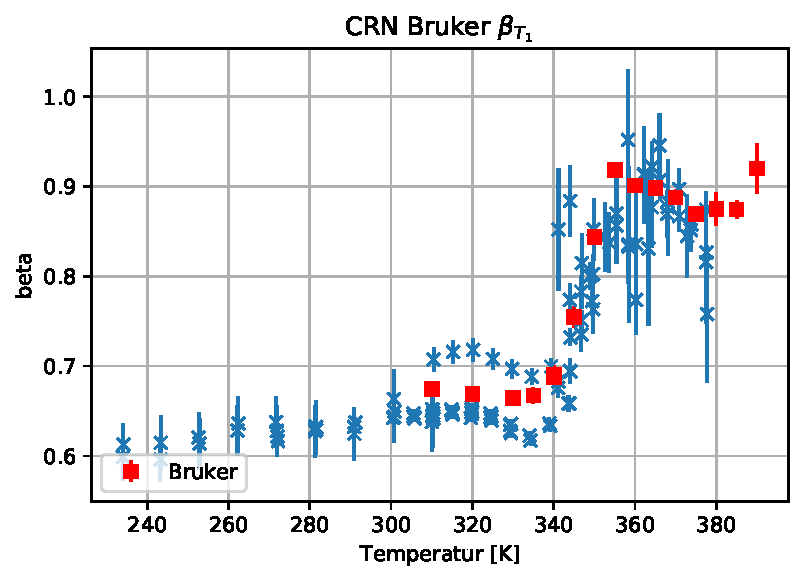
\includegraphics[width=\textwidth]{graphics/plots/BRUKER/bruker_t1beta.pdf}
	\end{center}
	\caption{Bruker $\beta{T_1}$} \label{fig:res:bruker_beta_t1}
\end{figure}

\begin{figure}
	\begin{center}
		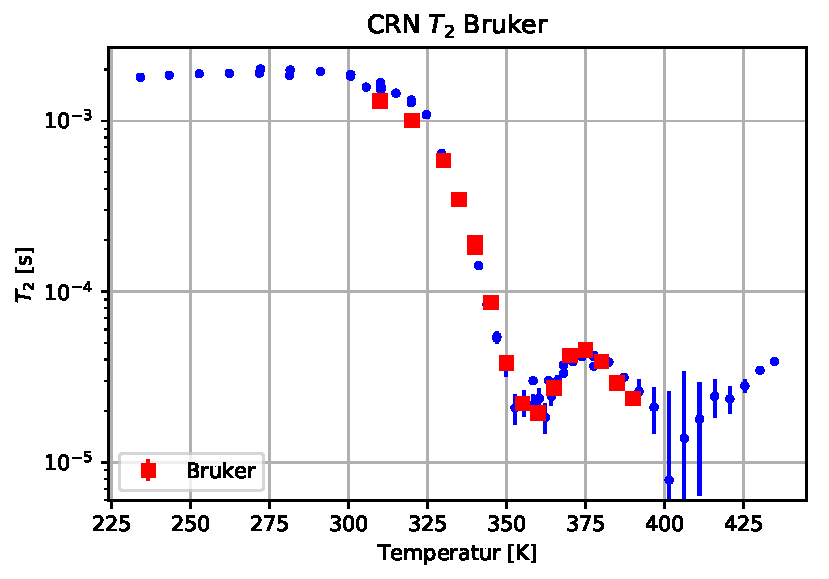
\includegraphics[width=\textwidth]{graphics/plots/BRUKER/bruker_t2.pdf}
	\end{center}
	\caption{Bruker $T_2$} \label{fig:res:bruker_t2}
\end{figure}
Die $T_2$-Werte und die dazugehörigen $\beta$ zeigen gute Übereinstimmung zu den anderen Daten auf, lediglich bei den hohen Temperaturen bei $\beta$ zeigen sich Abweichungen. Dies könnte der schlechten Datenqualität der Daten vom $\SI{300}{MHz}$-Spektrometer geschuldet sein.
\begin{figure}
	\begin{center}
		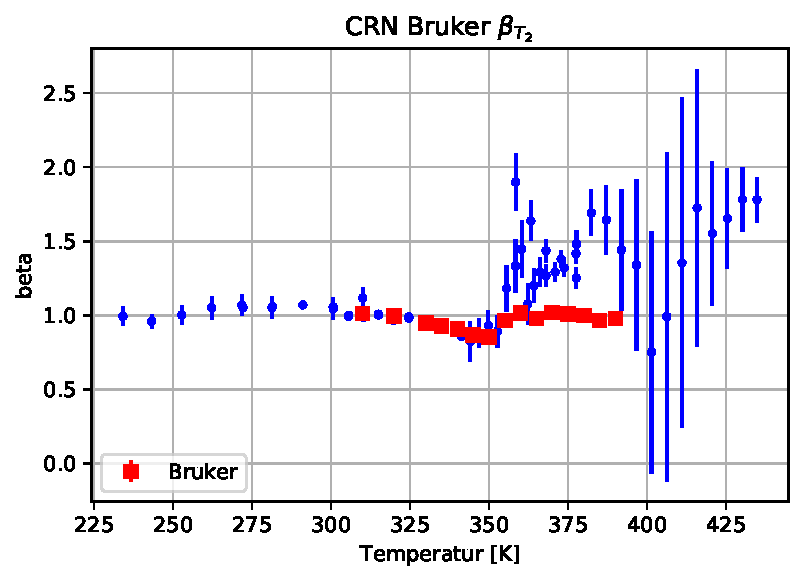
\includegraphics[width=\textwidth]{graphics/plots/BRUKER/bruker_t2beta.pdf}
	\end{center}
	\caption{Bruker $\beta{T_2}$} \label{fig:res:bruker_beta_t2}
\end{figure}

\begin{figure}
	\begin{center}
		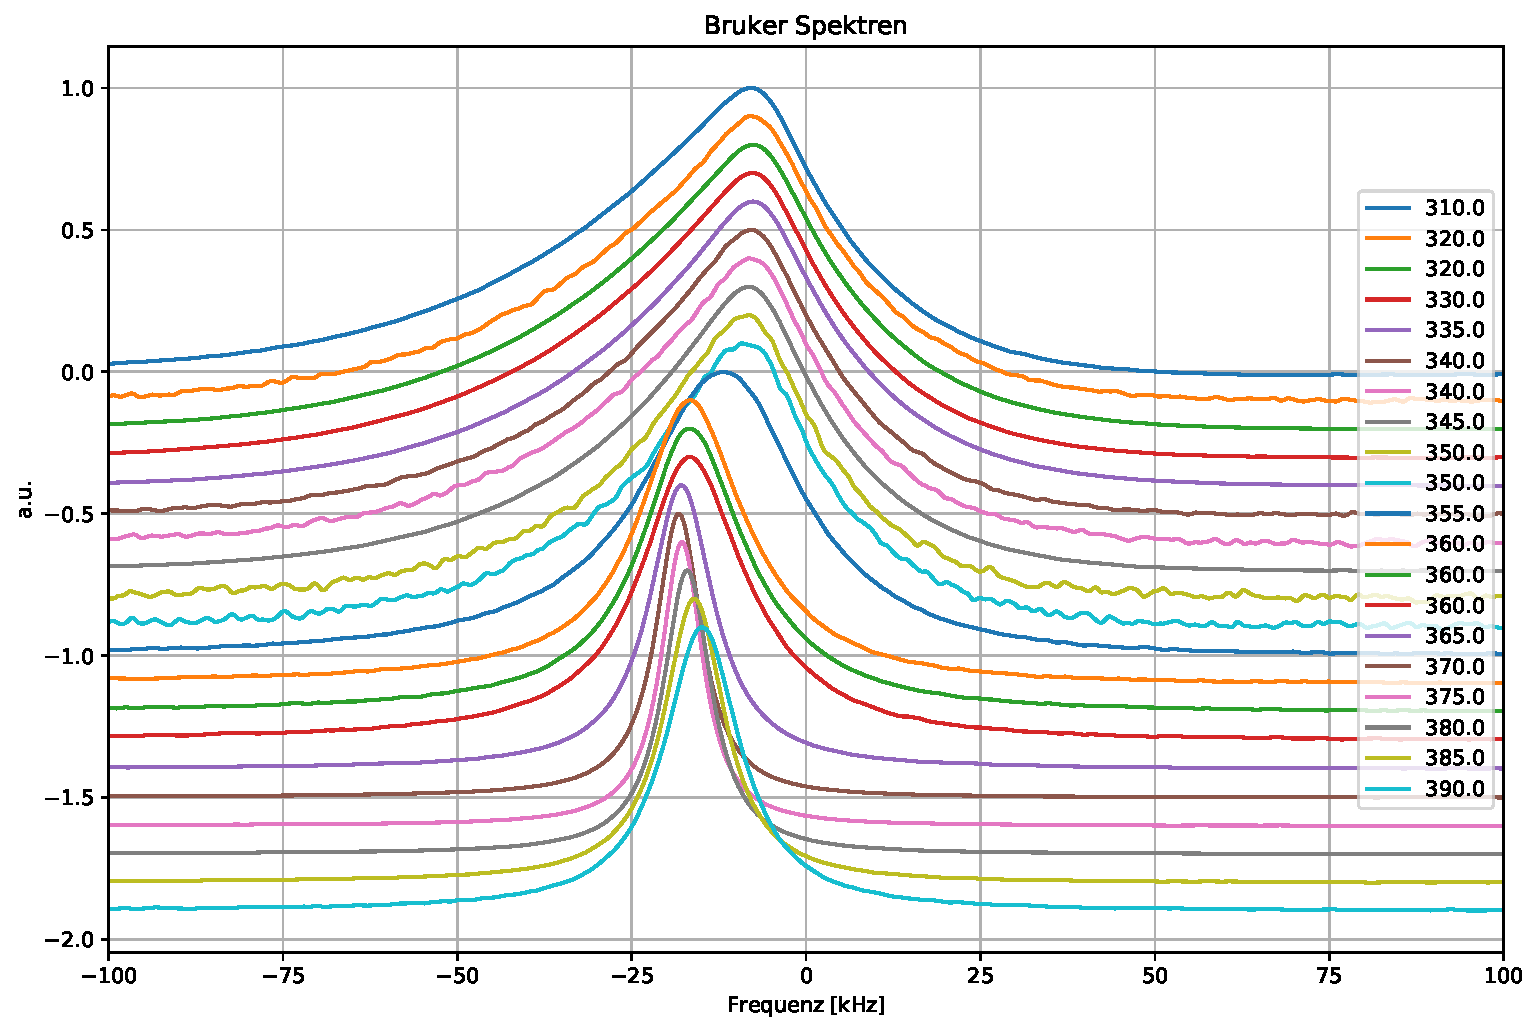
\includegraphics[width=\textwidth]{graphics/plots/BRUKER/bruker_lineshape.pdf}
	\end{center}
	\caption{Bruker Linienform} \label{fig:res:bruker_linienform}
\end{figure}
Die Linienform gleicht den der anderen Daten. Es ist die gute Qualität der Daten zu beachten.

\begin{figure}
	\begin{center}
		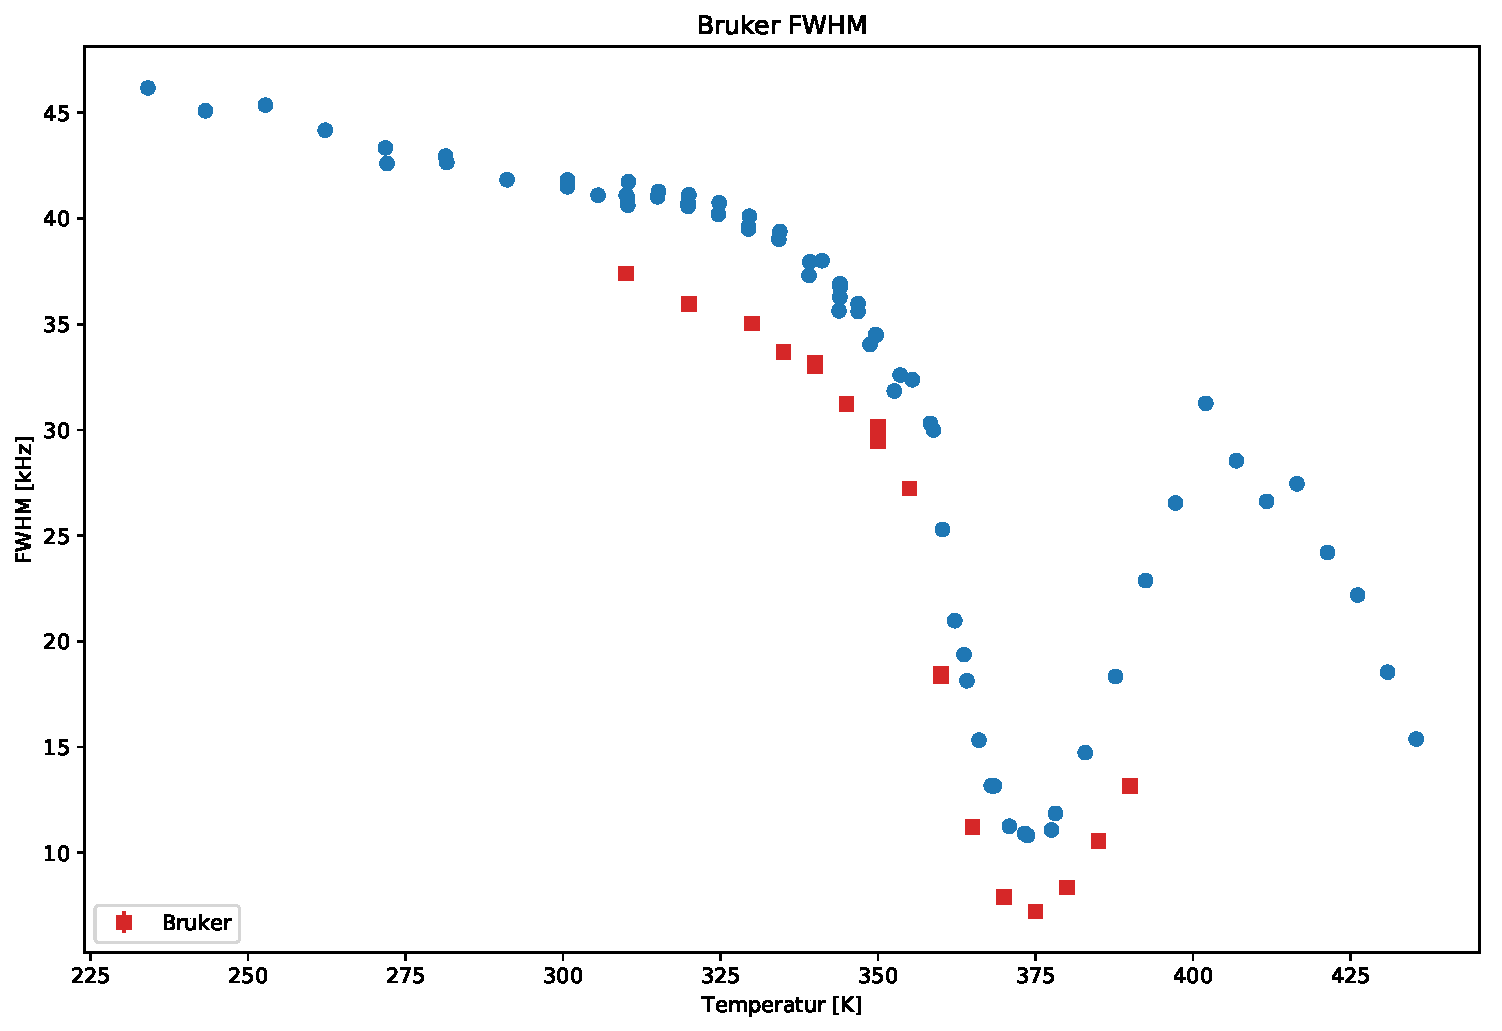
\includegraphics[width=\textwidth]{graphics/plots/BRUKER/bruker_fwhm.pdf}
	\end{center}
	\caption{Bruker FWHM} \label{fig:res:bruker_fwhm}
\end{figure}
Es gibt Abweichungen bei den Halbwertsbreiten. Es wäre aufgrund der Larmorfrequenzen (und der larmorfrequenzabhängigkeit des Quadrupol-WW) ein Verhältnis von 4:3 zu erwarten, was aber nicht ganz zutrifft. Messungen an einem $\SI{600}{MHz}$-Spektrometer wären hilfreich um Aussagen über die chemische Verschiebung machen zu können.

\begin{figure}
	\begin{center}
		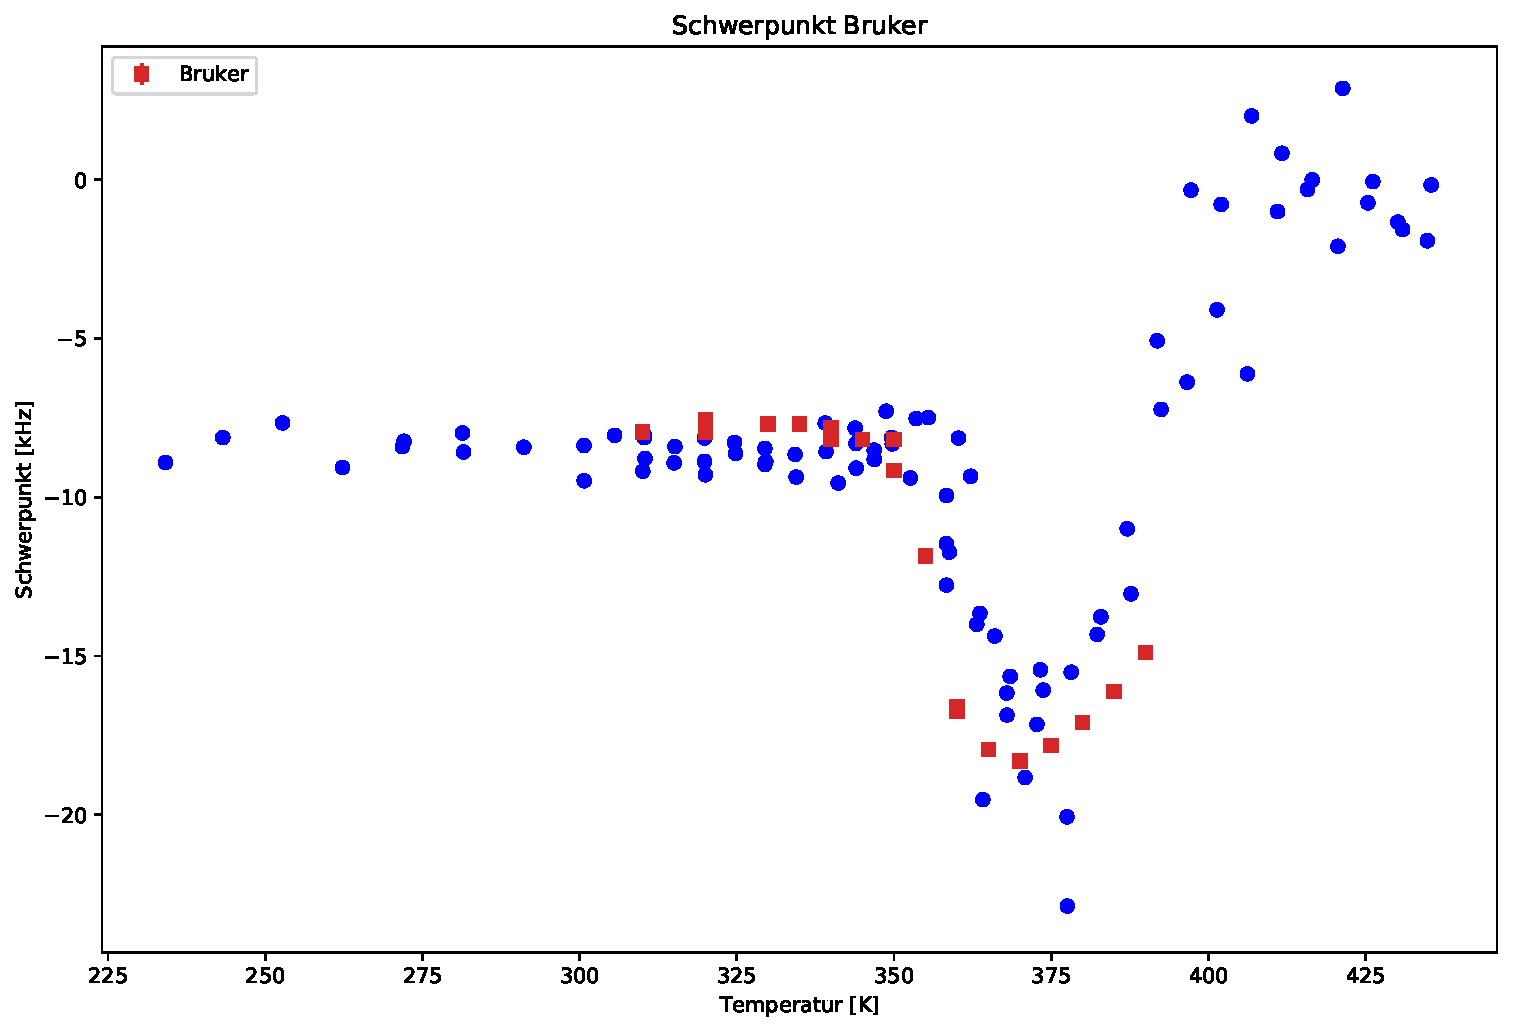
\includegraphics[width=\textwidth]{graphics/plots/BRUKER/bruker_mean.pdf} 
	\end{center}
	\caption{Bruker Schwerpunkt} \label{fig:res:bruker_mean}
\end{figure}





\section{Theoretische Beschreibung experimenteller CRN-Daten} \label{section:theo:daten}


Es wurde untersucht, ob vorliegende gemessenen Daten mit den beschriebenen Theorien in Einklang gebracht werden können. Dafür wurden die Daten zu $T_1$, zu Spektren untersucht; die $T_1$-Daten stammen dabei aus Messungen von C. Zürn \cite{zuern_paper} an einer 2Ca(NO$_3$)$_2$-3RbNO$_3$-Probe, während alle weiteren Daten mit der von Zürn verwendeten Probe im Rahmen dieser Masterarbeit aufgenommen wurden.

Um eine Übereinstimmung zur Theorie feststellen zu können, müssen sich alle Datensätze mit dem gleichen Satz geteilter Parameter beschreiben lassen. Im Falle der Spektraldichte $J(\omega)$ sind dies $C_Q$ und $\tau_{co}$; für $J_{CC}$ und $J_{CD}$ sind $\alpha$ bzw. $\gamma$ zusätzliche Parameter.

Nach \cite{PIMENOV199793} wird für CRN für die Korrelationszeit ein Vogel-Fulcher-Gesetz
\begin{align}
	\tau_c = \tau_{co} \exp \left( \frac{D T_\text{VF}}{T-T_\text{VF}} \right) 
\end{align}
mit dem strength index $D = \SI{3.5}{}$, der Vogel-Fulcher-Temperatur $T_\text{VF} = \SI{294}{K}$ und dem Frequenzfaktor $\tau_{co} = \SI{5.1e-14}{s}$ (der beim Vergleich mit den Daten dennoch als freier Parameter angesehen werden soll um dem Fit eine größtmögliche Flexibilität zu erlauben) angenommen.

\begin{wrapfigure}{r}{0.5\textwidth}
	\vspace{-20pt}
	\begin{center}
		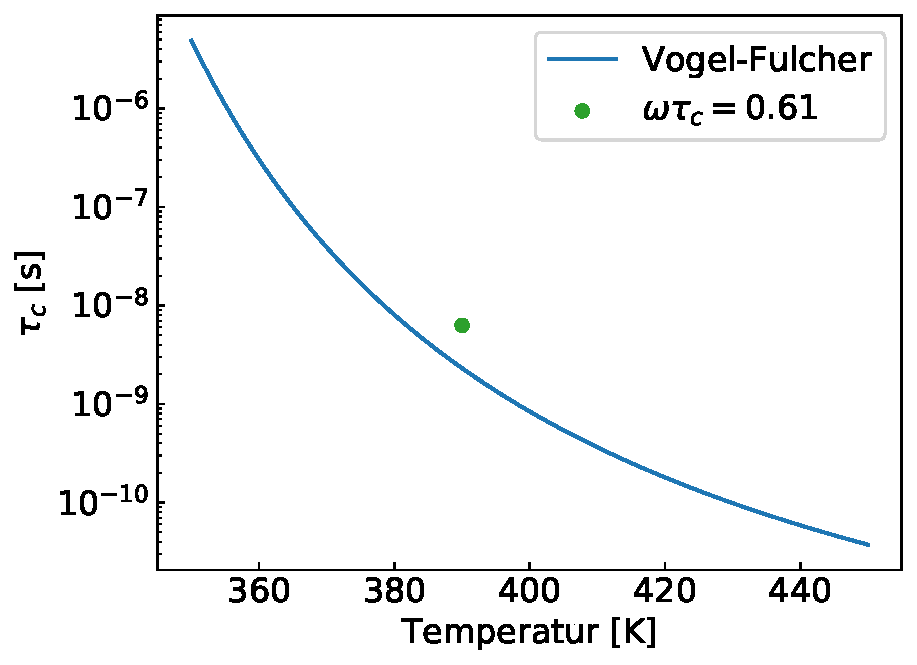
\includegraphics[width=0.49\textwidth]{graphics/zwischenbericht/tau_c_arrhenius_vogel_fulcher.pdf}
	\end{center}
	\vspace{-20pt}
	\caption{Vergleich von Korrelationszeiten basierend auf Vogel-Fulcher-Gesetz \label{fig:korrelationszeiten}}
\end{wrapfigure}
Am $T_1$-Minimum nach Gleichung \eqref{eqn:bpp} gilt $\omega \tau_c \approx \SI{0.61}{}$ \cite[S. 629]{omegatau061}. Das $T_1$-Minimum kann in den Daten bei etwa $T_\text{min} = \SI{390}{K}$ gefunden werden; die Larmorfrequenz liegt bei $\omega_L = \SI{97.1722}{MHz}$, was bedeutet, dass bei $T_\text{min}$ gilt $\tau_c \approx \frac{\SI{0.61}{}}{\omega_L} \approx \SI{6.28}{\nano s}$. Vergleicht man das Vogel-Fulcher-Gesetz mit diesem Punkt, lässt sich erkennen, dass eine gute Übereinstimmung vorliegt.


Die aufgenommenen Daten unterstützen eine biexponentielle Interpretation wie in \eqref{eqn:trans_relax} nur schwerlich, daher wurde lediglich der deutlich zu beobachtende Anteil des Zentralübergangs, $\Delta_c$ und $\omega_c^{(2)}$, für die entsprechenden FWHM- bzw. Schwerpunkts-Daten betrachtet. Für die $T_1$-Daten wird Formel \eqref{eqn:bpp} verwendet. Um einen Ausgangspunkt für die Analyse zu schaffen, wurden alle Fits per Hand erstellt, wobei durch das Ändern der Parameter versucht wurde eine möglichst gute Übereinstimmung zu erreichen.

Für die Spektraldichte $J(\omega)$ kann, wie in Abbildung \ref{fig:triple_vergleich} zu sehen, mit $\eta^2 = 42 - 24 \sqrt{3} \approx \SI{0.43}{}$ \cite{caer} und den Parametern $C_Q = \SI{3e6}{Hz}$ und $\tau_c = \SI{3.9e-14}{s}$ eine vergleichsweise gute Übereinstimmung für die $T_1$-Werte erreicht werden, die Flanken unterscheiden sich jedoch deutlich. Die Abweichungen der FWHM-Werten und der Schwerpunkte sind mit einem Faktor von etwa 4 bzw. etwa 2 bedeutend.
\begin{figure}[htbp]
	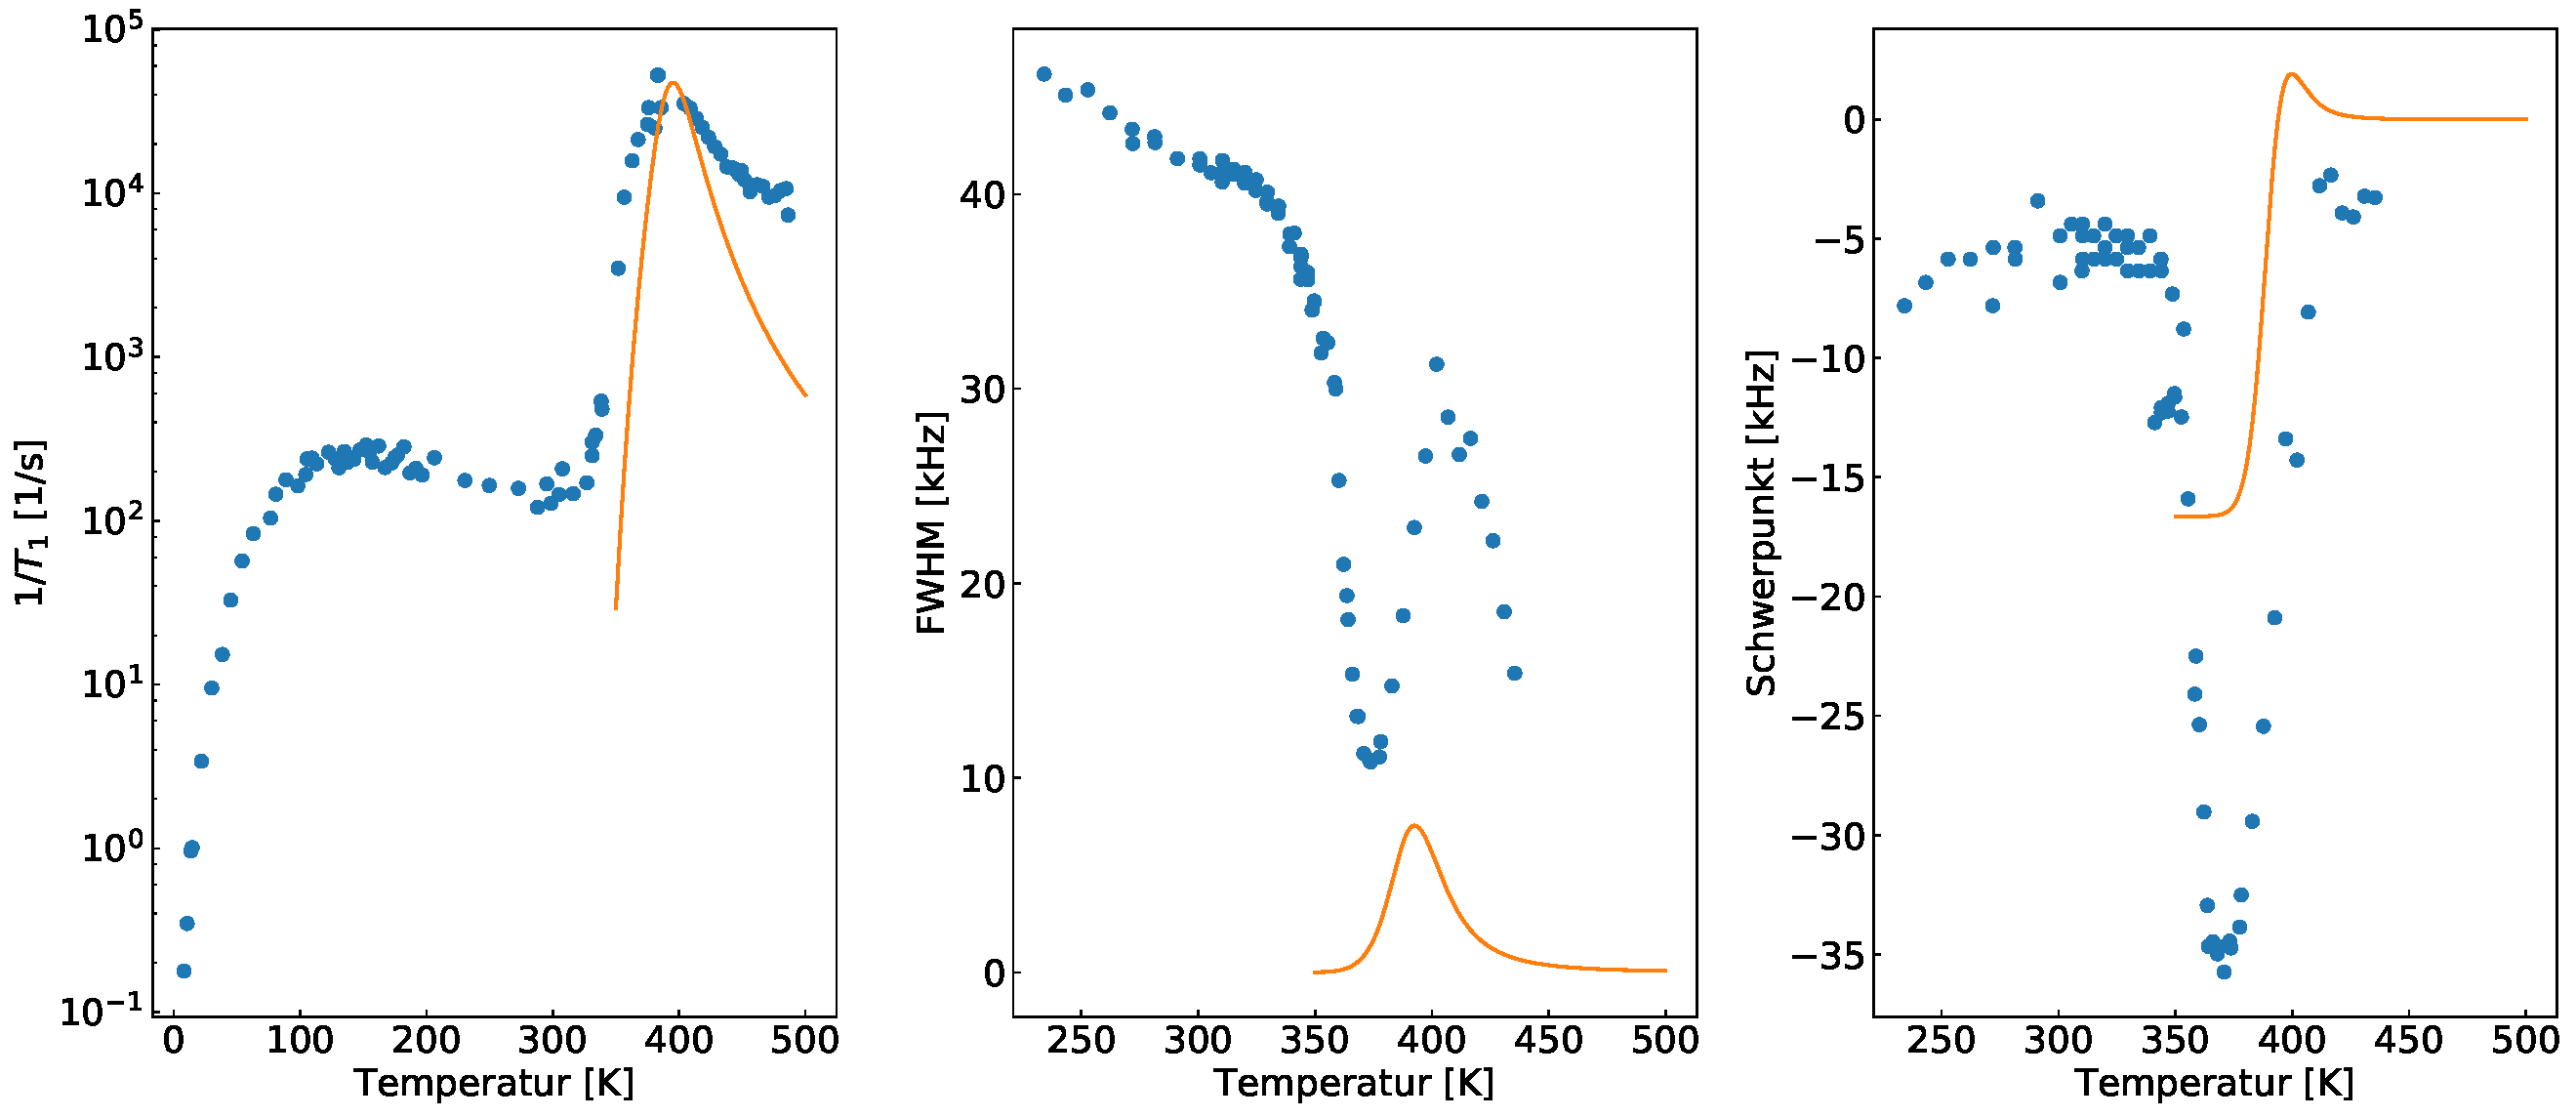
\includegraphics[width=\textwidth]{graphics/zwischenbericht/J_fertig.pdf}
	\caption{Vergleich der $T_1$-, FWHM- und Schwerpunkts-Daten (in blau) und der angepassten Theoriekurven (in orange). \label{fig:triple_vergleich}}
\end{figure}

Eine mögliche Erklärung für die Abweichung der FWHM-Werte könnte sein, dass in diesem Fall nicht, wie nach Formel \eqref{eqn:fwhm}, nur $T_2$, sondern auch das bei Temperaturen um $\SI{400}{K}$ mit etwa $\SI{50}{\micro s}$ äußerst kurze $T_1$ zur Verbreiterung des Spektrums und damit zu dessen FWHM-Werten beiträgt. Erste Versuche, den Effekt der $T_1$-Relaxation aus dem Spektrum herauszurechnen, scheinen vielversprechend. Für die Abweichungen der Schwerpunkts-Daten von der Theorie steht eine entsprechende Erklärung noch aus.

Aus diesem Grund jedoch soll für die Spektraldichten $J_{CC}$ und $J_{CD}$ die FWHM-Werte zunächst nicht betrachtet werden. Gleiches gilt für den Schwerpunkt, da die entsprechenden Imaginärteile der Spektraldichten, $Q_{CC}$ und $Q_{CD}$, nicht zur Verfügung stehen.

Für die Parameter $C_Q = \SI{2.85e6}{Hz}$, $\tau_c = \SI{7e-15}{s}$ und $\alpha = \SI{0.38}{}$ kann mit der Spektraldichte $J_{CC}$ in diesem Temperaturbereich eine noch bessere Übereinstimmung zu den $T_1$-Daten erzielt werden, für die Parameter $C_Q = \SI{2.7e6}{Hz}$, $\tau_c = \SI{4.4e-14}{s}$ und $\gamma = \SI{0.66}{}$ erreicht die Spektraldichte $J_{CD}$ eine leicht bessere Übereinstimmung als die Spektraldichte $J$; die entsprechenden Plots sind in Abbildung \ref{fig:j_cc_j_cd} zu finden.
\begin{figure}[H]
	\centering
	\begin{subfigure}{0.49\textwidth}
		\centering
		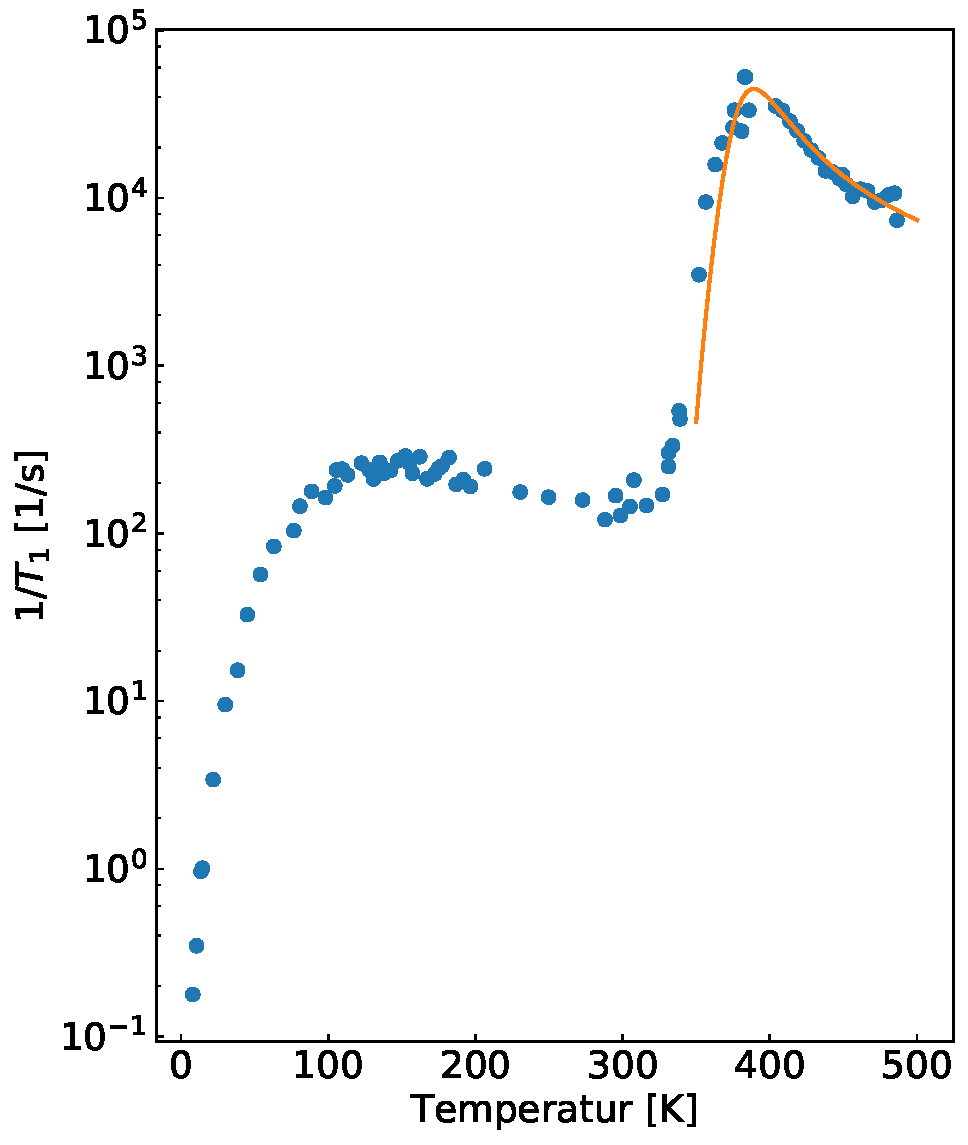
\includegraphics[width=0.95\textwidth]{graphics/zwischenbericht/J_cc.pdf}
	\end{subfigure}%
	\begin{subfigure}{0.49\textwidth}
		\centering
		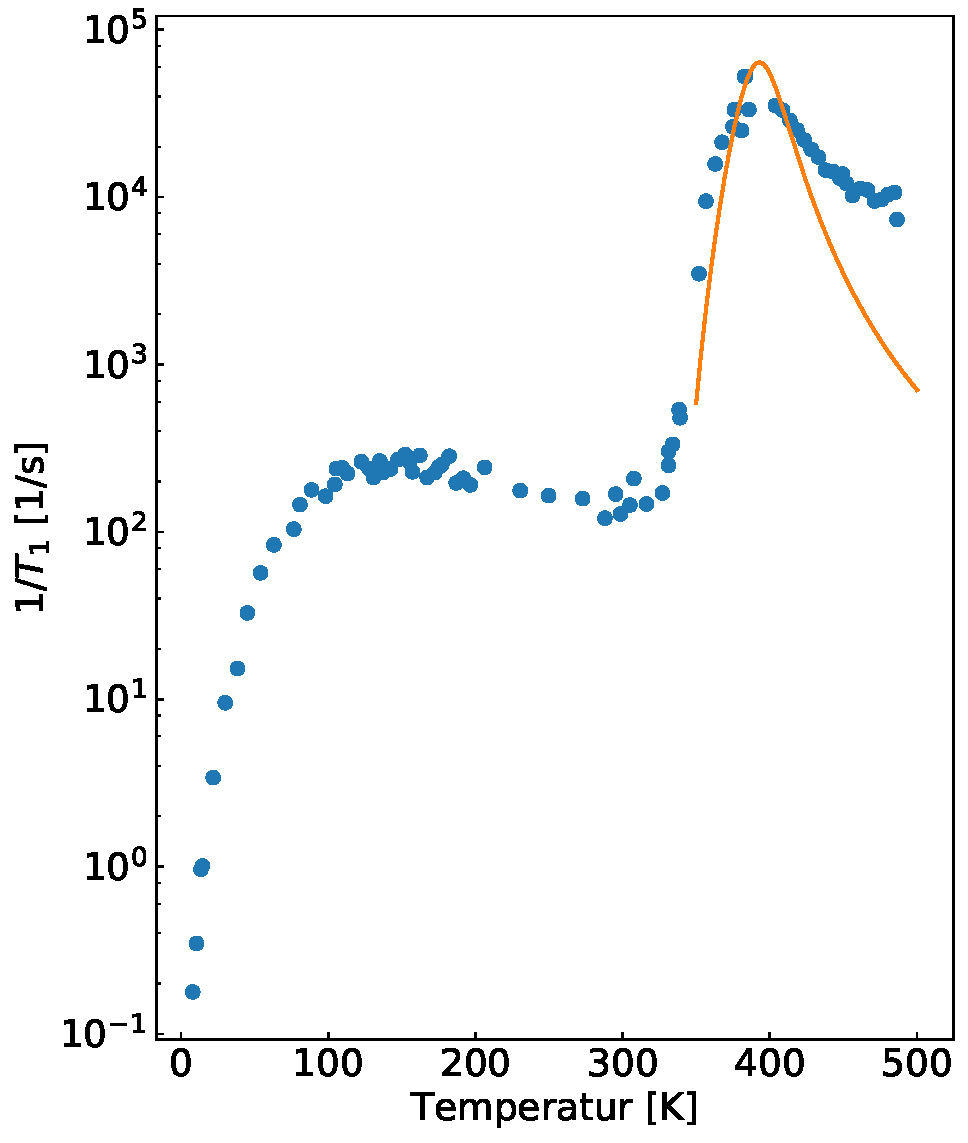
\includegraphics[width=0.95\textwidth]{graphics/zwischenbericht/J_cd.pdf}
	\end{subfigure}
	\caption{Spektraldichten $J_{CC}$ (links) und $J_{CD}$ (rechts), angepasst an die Daten}
	\label{fig:j_cc_j_cd}
\end{figure}

Die nächsten Schritte in dieser Untersuchung sollen darin bestehen, die Auswirkungen der $T_1$-Relaxation auf die Spektrums-Breite zu bestimmen und schlussendlich zu ergründen, ob sich die Messdaten sich mit diesen Theorien zufriedenstellend erklären lassen.


